% Options for packages loaded elsewhere
\PassOptionsToPackage{unicode}{hyperref}
\PassOptionsToPackage{hyphens}{url}
\PassOptionsToPackage{dvipsnames,svgnames,x11names}{xcolor}
%
\documentclass[
  11pt,
]{krantz}
\usepackage{amsmath,amssymb}
\usepackage{lmodern}
\usepackage{iftex}
\ifPDFTeX
  \usepackage[T1]{fontenc}
  \usepackage[utf8]{inputenc}
  \usepackage{textcomp} % provide euro and other symbols
\else % if luatex or xetex
  \usepackage{unicode-math}
  \defaultfontfeatures{Scale=MatchLowercase}
  \defaultfontfeatures[\rmfamily]{Ligatures=TeX,Scale=1}
  \setmonofont[Scale=0.775]{MesloLGS NF}
\fi
% Use upquote if available, for straight quotes in verbatim environments
\IfFileExists{upquote.sty}{\usepackage{upquote}}{}
\IfFileExists{microtype.sty}{% use microtype if available
  \usepackage[]{microtype}
  \UseMicrotypeSet[protrusion]{basicmath} % disable protrusion for tt fonts
}{}
\makeatletter
\@ifundefined{KOMAClassName}{% if non-KOMA class
  \IfFileExists{parskip.sty}{%
    \usepackage{parskip}
  }{% else
    \setlength{\parindent}{0pt}
    \setlength{\parskip}{6pt plus 2pt minus 1pt}}
}{% if KOMA class
  \KOMAoptions{parskip=half}}
\makeatother
\usepackage{xcolor}
\IfFileExists{xurl.sty}{\usepackage{xurl}}{} % add URL line breaks if available
\IfFileExists{bookmark.sty}{\usepackage{bookmark}}{\usepackage{hyperref}}
\hypersetup{
  pdftitle={Data Science per psicologi},
  pdfauthor={Corrado Caudek},
  colorlinks=true,
  linkcolor={Maroon},
  filecolor={Maroon},
  citecolor={Blue},
  urlcolor={Blue},
  pdfcreator={LaTeX via pandoc}}
\urlstyle{same} % disable monospaced font for URLs
\usepackage{color}
\usepackage{fancyvrb}
\newcommand{\VerbBar}{|}
\newcommand{\VERB}{\Verb[commandchars=\\\{\}]}
\DefineVerbatimEnvironment{Highlighting}{Verbatim}{commandchars=\\\{\}}
% Add ',fontsize=\small' for more characters per line
\usepackage{framed}
\definecolor{shadecolor}{RGB}{248,248,248}
\newenvironment{Shaded}{\begin{snugshade}}{\end{snugshade}}
\newcommand{\AlertTok}[1]{\textcolor[rgb]{0.33,0.33,0.33}{#1}}
\newcommand{\AnnotationTok}[1]{\textcolor[rgb]{0.37,0.37,0.37}{\textbf{\textit{#1}}}}
\newcommand{\AttributeTok}[1]{\textcolor[rgb]{0.61,0.61,0.61}{#1}}
\newcommand{\BaseNTok}[1]{\textcolor[rgb]{0.06,0.06,0.06}{#1}}
\newcommand{\BuiltInTok}[1]{#1}
\newcommand{\CharTok}[1]{\textcolor[rgb]{0.5,0.5,0.5}{#1}}
\newcommand{\CommentTok}[1]{\textcolor[rgb]{0.37,0.37,0.37}{\textit{#1}}}
\newcommand{\CommentVarTok}[1]{\textcolor[rgb]{0.37,0.37,0.37}{\textbf{\textit{#1}}}}
\newcommand{\ConstantTok}[1]{\textcolor[rgb]{0,0,0}{#1}}
\newcommand{\ControlFlowTok}[1]{\textcolor[rgb]{0.27,0.27,0.27}{\textbf{#1}}}
\newcommand{\DataTypeTok}[1]{\textcolor[rgb]{0.27,0.27,0.27}{#1}}
\newcommand{\DecValTok}[1]{\textcolor[rgb]{0.06,0.06,0.06}{#1}}
\newcommand{\DocumentationTok}[1]{\textcolor[rgb]{0.37,0.37,0.37}{\textbf{\textit{#1}}}}
\newcommand{\ErrorTok}[1]{\textcolor[rgb]{0.14,0.14,0.14}{\textbf{#1}}}
\newcommand{\ExtensionTok}[1]{#1}
\newcommand{\FloatTok}[1]{\textcolor[rgb]{0.06,0.06,0.06}{#1}}
\newcommand{\FunctionTok}[1]{\textcolor[rgb]{0,0,0}{#1}}
\newcommand{\ImportTok}[1]{#1}
\newcommand{\InformationTok}[1]{\textcolor[rgb]{0.37,0.37,0.37}{\textbf{\textit{#1}}}}
\newcommand{\KeywordTok}[1]{\textcolor[rgb]{0.27,0.27,0.27}{\textbf{#1}}}
\newcommand{\NormalTok}[1]{#1}
\newcommand{\OperatorTok}[1]{\textcolor[rgb]{0.43,0.43,0.43}{\textbf{#1}}}
\newcommand{\OtherTok}[1]{\textcolor[rgb]{0.37,0.37,0.37}{#1}}
\newcommand{\PreprocessorTok}[1]{\textcolor[rgb]{0.37,0.37,0.37}{\textit{#1}}}
\newcommand{\RegionMarkerTok}[1]{#1}
\newcommand{\SpecialCharTok}[1]{\textcolor[rgb]{0,0,0}{#1}}
\newcommand{\SpecialStringTok}[1]{\textcolor[rgb]{0.5,0.5,0.5}{#1}}
\newcommand{\StringTok}[1]{\textcolor[rgb]{0.5,0.5,0.5}{#1}}
\newcommand{\VariableTok}[1]{\textcolor[rgb]{0,0,0}{#1}}
\newcommand{\VerbatimStringTok}[1]{\textcolor[rgb]{0.5,0.5,0.5}{#1}}
\newcommand{\WarningTok}[1]{\textcolor[rgb]{0.37,0.37,0.37}{\textbf{\textit{#1}}}}
\usepackage{longtable,booktabs,array}
\usepackage{calc} % for calculating minipage widths
% Correct order of tables after \paragraph or \subparagraph
\usepackage{etoolbox}
\makeatletter
\patchcmd\longtable{\par}{\if@noskipsec\mbox{}\fi\par}{}{}
\makeatother
% Allow footnotes in longtable head/foot
\IfFileExists{footnotehyper.sty}{\usepackage{footnotehyper}}{\usepackage{footnote}}
\makesavenoteenv{longtable}
\usepackage{graphicx}
\makeatletter
\def\maxwidth{\ifdim\Gin@nat@width>\linewidth\linewidth\else\Gin@nat@width\fi}
\def\maxheight{\ifdim\Gin@nat@height>\textheight\textheight\else\Gin@nat@height\fi}
\makeatother
% Scale images if necessary, so that they will not overflow the page
% margins by default, and it is still possible to overwrite the defaults
% using explicit options in \includegraphics[width, height, ...]{}
\setkeys{Gin}{width=\maxwidth,height=\maxheight,keepaspectratio}
% Set default figure placement to htbp
\makeatletter
\def\fps@figure{htbp}
\makeatother
\setlength{\emergencystretch}{3em} % prevent overfull lines
\providecommand{\tightlist}{%
  \setlength{\itemsep}{0pt}\setlength{\parskip}{0pt}}
\setcounter{secnumdepth}{5}
\defaultfontfeatures{Scale=MatchLowercase}

\usepackage{booktabs}
\usepackage{longtable}
\usepackage[bf,singlelinecheck=off]{caption}

\usepackage{framed,color}
\definecolor{shadecolor}{RGB}{248,248,248}

\renewcommand{\textfraction}{0.05}
\renewcommand{\topfraction}{0.8}
\renewcommand{\bottomfraction}{0.8}
\renewcommand{\floatpagefraction}{0.75}

\renewenvironment{quote}{\begin{VF}}{\end{VF}}
\let\oldhref\href
\renewcommand{\href}[2]{#2\footnote{\url{#1}}}

\ifxetex
  \usepackage{letltxmacro}
  \setlength{\XeTeXLinkMargin}{1pt}
  \LetLtxMacro\SavedIncludeGraphics\includegraphics
  \def\includegraphics#1#{% #1 catches optional stuff (star/opt. arg.)
    \IncludeGraphicsAux{#1}%
  }%
  \newcommand*{\IncludeGraphicsAux}[2]{%
    \XeTeXLinkBox{%
      \SavedIncludeGraphics#1{#2}%
    }%
  }%
\fi

\makeatletter
\newenvironment{kframe}{%
\medskip{}
\setlength{\fboxsep}{.8em}
 \def\at@end@of@kframe{}%
 \ifinner\ifhmode%
  \def\at@end@of@kframe{\end{minipage}}%
  \begin{minipage}{\columnwidth}%
 \fi\fi%
 \def\FrameCommand##1{\hskip\@totalleftmargin \hskip-\fboxsep
 \colorbox{shadecolor}{##1}\hskip-\fboxsep
     % There is no \\@totalrightmargin, so:
     \hskip-\linewidth \hskip-\@totalleftmargin \hskip\columnwidth}%
 \MakeFramed {\advance\hsize-\width
   \@totalleftmargin\z@ \linewidth\hsize
   \@setminipage}}%
 {\par\unskip\endMakeFramed%
 \at@end@of@kframe}
\makeatother

\renewenvironment{Shaded}{\begin{kframe}}{\end{kframe}}

\usepackage{makeidx}
\makeindex

\urlstyle{tt}

\usepackage{amsthm}
\makeatletter
\def\thm@space@setup{%
  \thm@preskip=8pt plus 2pt minus 4pt
  \thm@postskip=\thm@preskip
}
\makeatother

\newcommand{\E}{\mathbb{E}} % Define expected value operator
\DeclareMathOperator{\Var}{\mathbb{V}} % Define variance operator
\DeclareMathOperator{\SD}{SD} % Define sd operator
\DeclareMathOperator{\Cov}{Cov} % Define covariance operator
\DeclareMathOperator{\Corr}{Corr} % Define correlation operator
\DeclareMathOperator{\Me}{Me} % Define mediane operator
\DeclareMathOperator{\Mo}{Mo} % Define mode operator
\DeclareMathOperator{\Bin}{Bin} % Define binomial operator
\DeclareMathOperator{\Bernoulli}{Bernoulli} % Define Bernoulli operator
\DeclareMathOperator{\Poi}{Poi} % Define Poisson operator
\DeclareMathOperator{\Uniform}{Uniform} % Define Uniform operator
\DeclareMathOperator{\Cauchy}{Cauchy} % Define Cauchy operator
\DeclareMathOperator{\elpd}{elpd} % Define elpd operator
\DeclareMathOperator{\lppd}{lppd} % Define lppd operator
\DeclareMathOperator{\LOO}{LOO} % Define LOO operator
\DeclareMathOperator{\Ber}{\mathscr{B}} % Define Bernoulli operator
\DeclareMathOperator{\B}{B} % beta function
% \mbox{B}(a, b) % beta function
% \mbox{Beta}(a, b) % beta distribution
\newcommand{\R}{\textsf{R}} % Define R programming language symbol
\newcommand{\Real}{\mathbb{R}} % Define real number operator
\newcommand{\Prob}{\mathscr{P}}
\newcommand{\indep}{\perp \!\!\! \perp}
\DeclareMathOperator{\argmin}{arg\,min} % thin space, limits on side in displays
\DeclareMathOperator{\argmax}{arg\,max} % no space, limits on side in displays

\raggedbottom % allow variable (ragged) site heights
\frenchspacing

\usepackage[
 labelfont=bf,
 font={small, it}
]{caption}
\usepackage{upquote} % print correct quotes in verbatim-environments
\usepackage{empheq}
\usepackage{xfrac}

\usepackage{polyglossia}
\setmainlanguage{italian}

% \DeclareMathSizes{10}{9}{7}{5}

\frontmatter
\ifLuaTeX
  \usepackage{selnolig}  % disable illegal ligatures
\fi
\usepackage[]{natbib}
\bibliographystyle{apalike}

\title{Data Science per psicologi}
\author{Corrado Caudek}
\date{2022-01-22}

\usepackage{amsthm}
\newtheorem{theorem}{Teorema}[chapter]
\newtheorem{lemma}{Lemma}[chapter]
\newtheorem{corollary}{Corollario}[chapter]
\newtheorem{proposition}{Proposizione}[chapter]
\newtheorem{conjecture}{Congettura}[chapter]
\theoremstyle{definition}
\newtheorem{definition}{Definizione}[chapter]
\theoremstyle{definition}
\newtheorem{example}{Esempio}[chapter]
\theoremstyle{definition}
\newtheorem{exercise}{Esercizio}[chapter]
\theoremstyle{definition}
\newtheorem{hypothesis}{Hypothesis}[chapter]
\theoremstyle{remark}
\newtheorem*{remark}{Osservazione}
\newtheorem*{solution}{Soluzione}
\begin{document}
\maketitle

\cleardoublepage\newpage\thispagestyle{empty}\null
% \cleardoublepage\newpage\thispagestyle{empty}\null
%\cleardoublepage\newpage
\thispagestyle{empty}
\begin{center}
\Large{Psicometria -- AA 2021/2022}

\vskip20pt

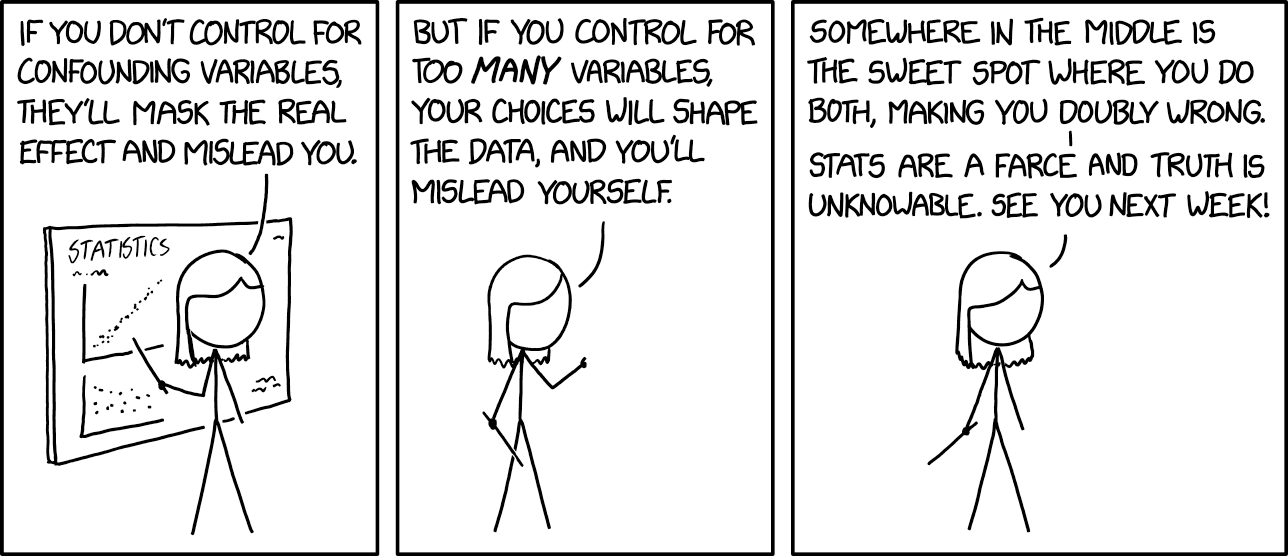
\includegraphics{images/confounding_variables.png}
\end{center}

\setlength{\abovedisplayskip}{-5pt}
\setlength{\abovedisplayshortskip}{-5pt}

{
\hypersetup{linkcolor=}
\setcounter{tocdepth}{2}
\tableofcontents
}
\listoffigures
\listoftables
\hypertarget{prefazione}{%
\chapter*{Prefazione}\label{prefazione}}


\emph{Data Science per psicologi} contiene il materiale delle lezioni dell'insegnamento di \emph{Psicometria B000286} (A.A. 2021/2022) rivolto agli studenti del primo anno del Corso di Laurea in Scienze e Tecniche Psicologiche dell'Università degli Studi di Firenze. \emph{Psicometria} si propone di fornire agli studenti un'introduzione all'analisi dei dati in psicologia. Le conoscenze/competenze che verranno sviluppate in questo insegnamento sono quelle della Data science, ovvero un insieme di conoscenze/competenze che si pongono all'intersezione tra statistica (ovvero, richiedono la capacità di comprendere teoremi statistici) e informatica (ovvero, richiedono la capacità di sapere utilizzare un software).

\hypertarget{la-psicologia-e-la-data-science}{%
\section*{La psicologia e la Data science}\label{la-psicologia-e-la-data-science}}


Sembra sensato spendere due parole su un tema che è importante per gli studenti: quello indicato dal titolo di questo Capitolo. È ovvio che agli studenti di psicologia la statistica non piace. Se piacesse, forse studierebbero Data science e non psicologia; ma non lo fanno. Di conseguenza, gli studenti di psicologia si chiedono: ``perché dobbiamo perdere tanto tempo a studiare queste cose quando in realtà quello che ci interessa è tutt'altro?'' Questa è una bella domanda.

C'è una ragione molto semplice che dovrebbe farci capire perché la Data science è così importante per la psicologia. Infatti, a ben pensarci, la psicologia è una disciplina intrinsecamente statistica, se per statistica intendiamo quella disciplina che studia la variazione delle caratteristiche degli individui nella popolazione. La psicologia studia \emph{gli individui} ed è proprio la variabilità inter- e intra-individuale ciò che vogliamo descrivere e, in certi casi, predire. In questo senso, la psicologia è molto diversa dall'ingegneria, per esempio. Le proprietà di un determinato ponte sotto certe condizioni, ad esempio, sono molto simili a quelle di un altro ponte, sotto le medesime condizioni. Quindi, per un ingegnere la statistica è poco importante: le proprietà dei materiali sono unicamente dipendenti dalla loro composizione e restano costanti. Ma lo stesso non può dirsi degli individui: ogni individuo è unico e cambia nel tempo. E le variazioni tra gli individui, e di un individuo nel tempo, sono l'oggetto di studio proprio della psicologia: è dunque chiaro che i problemi che la psicologia si pone sono molto diversi da quelli affrontati, per esempio, dagli ingegneri. Questa è la ragione per cui abbiamo tanto bisogno della Data science in psicologia: perché la Data science ci consente di descrivere la variazione e il cambiamento. E queste sono appunto le caratteristiche di base dei fenomeni psicologici.

Sono sicuro che, leggendo queste righe, a molti studenti sarà venuta in mente la seguente domanda: perché non chiediamo a qualche esperto di fare il ``lavoro sporco'' (ovvero le analisi statistiche) per noi, mentre noi (gli psicologi) ci occupiamo solo di ciò che ci interessa, ovvero dei problemi psicologici slegati dai dettagli ``tecnici'' della Data science? La risposta a questa domanda è che non è possibile progettare uno studio psicologico sensato senza avere almeno una comprensione rudimentale della Data science. Le tematiche della Data science non possono essere ignorate né dai ricercatori in psicologia né da coloro che svolgono la professione di psicologo al di fuori dell'Università. Infatti, anche i professionisti al di fuori dall'università non possono fare a meno di leggere la letteratura psicologica più recente: il continuo aggiornamento delle conoscenze è infatti richiesto dalla deontologia della professione. Ma per potere fare questo è necessario conoscere un bel po' di Data science! Basta aprire a caso una rivista specialistica di psicologia per rendersi conto di quanto ciò sia vero: gli articoli che riportano i risultati delle ricerche psicologiche sono zeppi di analisi statistiche e di modelli formali. E la comprensione della letteratura psicologica rappresenta un requisito minimo nel bagaglio professionale dello psicologo.

Le considerazioni precedenti cercano di chiarire il seguente punto: la Data science non è qualcosa da studiare a malincuore, in un singolo insegnamento universitario, per poi poterla tranquillamente dimenticare. Nel bene e nel male, gli psicologi usano gli strumenti della Data science in tantissimi ambiti della loro attività professionale: in particolare quando costruiscono, somministrano e interpretano i test psicometrici. È dunque chiaro che possedere delle solide basi di Data science è un tassello imprescindibile del bagaglio professionale dello psicologo. In questo insegnamento verrano trattati i temi base della Data science e verrà adottato un punto di vista bayesiano, che corrisponde all'approccio più recente e sempre più diffuso in psicologia.

\hypertarget{come-studiare}{%
\section*{Come studiare}\label{come-studiare}}


Il giusto metodo di studio per prepararsi all'esame di Psicometria è quello di seguire attivamente le lezioni, assimilare i concetti via via che essi vengono presentati e verificare in autonomia le procedure presentate a lezione. Incoraggio gli studenti a farmi domande per chiarire ciò che non è stato capito appieno. Incoraggio gli studenti a utilizzare i forum attivi su Moodle e, soprattutto, a svolgere gli esercizi proposti su Moodle. I problemi forniti su Moodle rappresentano il livello di difficoltà richiesto per superare l'esame e consentono allo studente di comprendere se le competenze sviluppate fino a quel punto sono sufficienti rispetto alle richieste dell'esame.

La prima fase dello studio, che è sicuramente individuale, è quella in cui è necessario acquisire le conoscenze teoriche relative ai problemi che saranno presentati all'esame. La seconda fase di studio, che può essere facilitata da scambi con altri e da incontri di gruppo, porta ad acquisire la capacità di applicare le conoscenze: è necessario capire come usare un software (\(\textsf{R}\)) per applicare i concetti statistici alla specifica situazione del problema che si vuole risolvere. Le due fasi non sono però separate: il saper fare molto spesso ci aiuta a capire meglio.

\hypertarget{sviluppare-un-metodo-di-studio-efficace}{%
\section*{Sviluppare un metodo di studio efficace}\label{sviluppare-un-metodo-di-studio-efficace}}


Avendo insegnato molte volte in passato un corso introduttivo di analisi dei dati ho notato nel corso degli anni che gli studenti con l'atteggiamento mentale che descriverò qui sotto generalmente ottengono ottimi risultati. Alcuni studenti sviluppano naturalmente questo approccio allo studio, ma altri hanno bisogno di fare uno sforzo per maturarlo. Fornisco qui sotto una breve descrizione del ``metodo di studio'' che, nella mia esperienza, è il più efficace per affrontare le richieste di questo insegnamento.

\begin{itemize}
\tightlist
\item
  Dedicate un tempo sufficiente al materiale di base, apparentemente facile; assicuratevi di averlo capito bene. Cercate le lacune nella vostra comprensione. Leggere presentazioni diverse dello stesso materiale (in libri o articoli diversi) può fornire nuove intuizioni.
\item
  Gli errori che facciamo sono i nostri migliori maestri. Istintivamente cerchiamo di dimenticare subito i nostri errori. Ma il miglior modo di imparare è apprendere dagli errori che commettiamo. In questo senso, una soluzione corretta è meno utile di una soluzione sbagliata. Quando commettiamo un errore questo ci fornisce un'informazione importante: ci fa capire qual è il materiale di studio sul quale dobbiamo ritornare e che dobbiamo capire meglio.
\item
  C'è ovviamente un aspetto ``psicologico'' nello studio. Quando un esercizio o problema ci sembra incomprensibile, la cosa migliore da fare è dire: ``mi arrendo'', ``non ho idea di cosa fare!''. Questo ci rilassa: ci siamo già arresi, quindi non abbiamo niente da perdere, non dobbiamo più preoccuparci. Ma non dobbiamo fermarci qui. Le cose ``migliori'' che faccio (se ci sono) le faccio quando non ho voglia di lavorare. Alle volte, quando c'è qualcosa che non so fare e non ho idea di come affontare, mi dico: ``oggi non ho proprio voglia di fare fatica'', non ho voglia di mettermi nello stato mentale per cui ``in 10 minuti devo risolvere il problema perché dopo devo fare altre cose''. Però ho voglia di \emph{divertirmi} con quel problema e allora mi dedico a qualche aspetto ``marginale'' del problema, che so come affrontare, oppure considero l'aspetto più difficile del problema, quello che non so come risolvere, ma invece di cercare di risolverlo, guardo come altre persone hanno affrontato problemi simili, opppure lo stesso problema in un altro contesto. Non mi pongo l'obiettivo ``risolvi il problema in 10 minuti'', ma invece quello di farmi un'idea ``generale'' del problema, o quello di capire un caso più specifico e più semplice del problema. Senza nessuna pressione. Infatti, in quel momento ho deciso di non lavorare (ovvero, di non fare fatica). Va benissimo se ``parto per la tangente'', ovvero se mi metto a leggere del materiale che sembra avere poco a che fare con il problema centrale (le nostre intuizioni e la nostra curiosità solitamente ci indirizzano sulla strada giusta). Quando faccio così, molto spesso trovo la soluzione del problema che mi ero posto e, paradossalmente, la trovo in un tempo minore di quello che, in precedenza, avevo dedicato a ``lavorare'' al problema. Allora perché non faccio sempre così? C'è ovviamente l'aspetto dei ``10 minuti'' che non è sempre facile da dimenticare. Sotto pressione, possiamo solo agire in maniera automatica, ovvero possiamo solo applicare qualcosa che già sappiamo fare. Ma se dobbiamo imparare qualcosa di nuovo, la pressione è un impedimento.
\item
  È utile farsi da soli delle domande sugli argomenti trattati, senza limitarsi a cercare di risolvere gli esercizi che vengono assegnati. Quando studio qualcosa mi viene in mente: ``se questo è vero, allora deve succedere quest'altra cosa''. Allora verifico se questo è vero, di solito con una simulazione. Se i risultati della simulazione sono quelli che mi aspetto, allora vuol dire che ho capito. Se i risultati sono diversi da quelli che mi aspettavo, allora mi rendo conto di non avere capito e ritorno indietro a studiare con più attenzione la teoria che pensavo di avere capito -- e ovviamente mi rendo conto che c'era un aspetto che avevo frainteso. Questo tipo di verifica è qualcosa che dobbiamo fare da soli, in prima persona: nessun altro può fare questo al posto nostro.
\item
  Non aspettatevi di capire tutto la prima volta che incontrate un argomento nuovo.\footnote{Ricordatevi inoltre che gli individui tendono a sottostimare la propria capacità di apprendere \citep{horn2021underestimating}.} È utile farsi una nota mentalmente delle lacune nella vostra comprensione e tornare su di esse in seguito per carcare di colmarle. L'atteggiamento naturale, quando non capiamo i dettagli di qualcosa, è quello di pensare: ``non importa, ho capito in maniera approssimativa questo punto, non devo preoccuparmi del resto''. Ma in realtà non è vero: se la nostra comprensione è superficiale, quando il problema verrà presentato in una nuova forma, non riusciremo a risolverlo. Per cui i dubbi che ci vengono quando studiamo qualcosa sono il nostro alleato più prezioso: ci dicono esattamente quali sono gli aspetti che dobbiamo approfondire per potere migliorare la nostra preparazione.
\item
  È utile sviluppare una visione d'insieme degli argomenti trattati, capire l'obiettivo generale che si vuole raggiungere e avere chiaro il contributo che i vari pezzi di informazione forniscono al raggiungimento di tale obiettivo. Questa organizzazione mentale del materiale di studio facilita la comprensione. È estremamente utile creare degli schemi di ciò che si sta studiando. Non aspettate che sia io a fornirvi un riepilogo di ciò che dovete imparare: sviluppate da soli tali schemi e tali riassunti.
\item
  Tutti noi dobbiamo imparare l'arte di trovare le informazioni, non solo nel caso di questo insegnamento. Quando vi trovate di fronte a qualcosa che non capite, o ottenete un oscuro messaggio di errore da un software, ricordatevi: ``Google is your friend''!
\end{itemize}

\begin{flushright}
Corrado Caudek\\
Marzo 2022 \end{flushright}

\mainmatter

\hypertarget{part-inferenza-statistica-bayesiana}{%
\part{Inferenza statistica bayesiana}\label{part-inferenza-statistica-bayesiana}}

\hypertarget{ch:intro-bayes-inference}{%
\chapter{Inferenza bayesiana}\label{ch:intro-bayes-inference}}

La moderna statistica bayesiana viene per lo più eseguita utilizzando un linguaggio di programmazione probabilistico implementato su computer. Ciò ha cambiato radicalmente il modo in cui venivano eseguite le statistiche bayesiane anche fin pochi decenni fa. La complessità dei modelli che possiamo costruire è aumentata e la barriera delle competenze matematiche e computazionali che sono richieste è diminuita. Inoltre, il processo di modellazione iterativa è diventato, sotto molti aspetti, molto più facile da eseguire. Anche se formulare modelli statistici complessi è diventato più facile che mai, la statistica è un campo pieno di sottigliezze che non scompaiono magicamente utilizzando potenti metodi computazionali. Pertanto, avere una buona preparazione sugli aspetti teorici, specialmente quelli rilevanti nella pratica, è estremamente utile per applicare efficacemente i metodi statistici.

\hypertarget{modellizzazione-bayesiana}{%
\section{Modellizzazione bayesiana}\label{modellizzazione-bayesiana}}

Seguendo \citep{martin2022bayesian}, possiamo descrivere il processo della modellazione bayesiana distinguendo 3 passaggi.

\begin{enumerate}
\def\labelenumi{\arabic{enumi}.}
\tightlist
\item
  Dati alcuni dati e alcune ipotesi su come questi dati potrebbero essere stati generati, progettiamo un modello combinando e trasformando variabili casuali.
\item
  Usiamo il teorema di Bayes per condizionare i nostri modelli ai dati disponibili. Chiamiamo questo processo ``inferenza'' e come risultato otteniamo una distribuzione a posteriori. Ci auguriamo che i dati riducano l'incertezza per i possibili valori dei parametri, sebbene questo non sia garantito per nessun modello bayesiano.
\item
  Critichiamo il modello verificando se il modello abbia senso utilizzando criteri diversi, inclusi i dati e la nostra conoscenza del dominio. Poiché generalmente siamo incerti sui modelli stessi, a volte confrontiamo diversi modelli.
\end{enumerate}

Questi 3 passaggi vengono eseguiti in modo iterativo e danno luogo a quello che si chiama un ``flusso di lavoro bayesiano'' (\emph{bayesian workflow}).

\begin{remark}
Un modello è uno strumento concettuale che viene utilizzato per risolvere uno specifico problema. In quanto tale, è generalmente più conveniente parlare dell'adeguatezza del modello a un dato problema che di determinare la sua intrinseca correttezza. I modelli esistono esclusivamente come l'ausilio per il raggiungimento di un qualche ulteriore obiettivo. Il problema che i modelli bayesiani cercano di risolvere è quello dell'inferenza\footnote{In termini colloquiali, l'inferenza può essere descritta come la capacità di giungere a conclusioni basate su evidenze e ragionamenti. L'inferenza bayesiana è una particolare forma di inferenza statistica basata sulla combinazione di distribuzioni di probabilità che ha il fine di ottenere altre distribuzioni di probabilità. Nello specifico, la regola di Bayes ci fornisce un metodo per giungere alla quantificazione della plausibilità di una teoria alla luce dei dati osservati.}.
\end{remark}

I modelli bayesiani, computazionali o meno, hanno due caratteristiche distintive:

\begin{itemize}
\tightlist
\item
  Le quantità incognite sono descritte utilizzando le distribuzioni di probabilità. Queste quantità incognite sono chiatame parametri.
\item
  Il teorema di Bayes viene utilizzato per aggiornare i valori dei parametri condizionati ai dati. Possiamo anche concepire questo processo come una riallocazione delle probabilità.
\end{itemize}

\hypertarget{inferenza-bayesiana-come-un-problema-inverso}{%
\section{Inferenza bayesiana come un problema inverso}\label{inferenza-bayesiana-come-un-problema-inverso}}

In questo capitolo ci focalizzeremo sul passaggio 2 descritto sopra. Nello specifico, descrivemo in dettaglio il significato dei tre i termini a destra del segno di uguale nella formula di Bayes: la distribuzione a priori e la funzione di verosimiglianza al numeratore, e la verosimiglianza marginale al denominatore.

\hypertarget{notazione}{%
\subsection{Notazione}\label{notazione}}

Per fissare la notazione, nel seguito \(y\) rappresenterà i dati e \(\theta\) rappresenterà i parametri incogniti di un modello statistico. Sia \(y\) che \(\theta\) saranno concepiti come delle variabili casuali.\footnote{Nell'approccio bayesiano si fa riferimento ad un modello probabilistico \(f(y \mid \theta)\) rappresentativo del fenomeno d'interesse noto a meno del valore assunto dal parametro (o dei parametri) che lo caratterizza. Si fa inoltre riferimento ad una distribuzione congiunta (di massa o di densità di probabilità) \(f(y, \theta)\). Entrambi gli argomenti della funzione \(y\) e \(\theta\) hanno natura di variabili casuali, laddove la nostra incertezza relativa a \(y\) è dovuta alla naturale variabilità del fenomeno indagato (\emph{variabilità aleatoria}), mentre la nostra incertezza relativa a \(\theta\) è dovuta alla mancata conoscenza del suo valore numerico (\emph{variabilità epistemica}).} Con \(x\) verranno invece denotate le quantità note, come ad esempio i predittori del modello lineare. Per rappresentare in un modo conciso i modelli probabilistici viene usata una notazione particolare. Ad esempio, invece di scrivere \(p(\theta) = \mbox{Beta}(1, 1)\) scriviamo \(\theta \sim \mbox{Beta}(1, 1)\). Il simbolo ``\(\sim\)'' viene spesso letto ``è distribuito come''. Possiamo anche pensare che significhi che \(\theta\) costituisce un campione casuale estratto dalla distribuzione Beta(1, 1). Allo stesso modo, ad esempio, la verosimiglianza del modello binomiale può essere scritta come \(y \sim \text{Bin}(n, \theta)\).

\hypertarget{funzioni-di-probabilituxe0}{%
\subsection{Funzioni di probabilità}\label{funzioni-di-probabilituxe0}}

Una caratteristica attraente della statistica bayesiana è che la nostra credenza ``a posteriori'' viene sempre descritta mediante una distribuzione. Questo fatto ci consente di fare affermazioni probabilistiche sui parametri, come ad esempio: ``la probabilità che un parametro sia positivo è 0.35''; oppure, ``il valore più probabile di \(\theta\) è 12 e abbiamo probabilità del 50\% che \(\theta\) sia compreso tra 10 e 15''. Inoltre, possiamo pensare alla distribuzione a posteriori come alla logica conseguenza della combinazione di un modello con i dati; quindi, abbiamo la garanzia che le affermazioni probabilistiche associate alla distribuzione a posteriori siano matematicamente coerenti. Dobbiamo solo ricordare che tutte queste belle proprietà matematiche sono valide solo nel mondo platonico delle idee dove esistono oggetti matematici come sfere, distribuzioni gaussiane e catene di Markov. Quando passiamo dalla purezza della matematica al disordine della matematica applicata al mondo reale, dobbiamo sempre tenere a mente che i nostri risultati sono condizionati, non solo dai dati, ma anche dai modelli. Di conseguenza, dati errati e/o modelli errati conducono facilmente a conclusioni prive di senso, anche se matematicamente coerenti. È dunque necessario conservare sempre una sana quota di scetticismo relativamente ai nostri dati, modelli e risultati \citep{martin2022bayesian}.

Avendo detto questo, nell'aggiornamento bayesiano (dai dati ai parametri) vengono utilizzate le seguenti distribuzioni di probabilità (o di massa di probabilità):

\begin{itemize}
\tightlist
\item
  la \emph{distribuzione a priori} \(p(\theta)\) --- la credenza iniziale (prima di avere osservato i dati \(Y = y\)) riguardo a \(\theta\);
\item
  la \emph{funzione di verosimiglianza} \(p(y \mid \theta)\) --- quanto sono compatibili i dati osservati \(Y = y\) con i diversi valori possibili di \(\theta\)?
\item
  la \emph{verosimiglianza marginale} \(p(y)\) --- costante di normalizzazione: qual è la probabilità complessiva di osservare i dati \(Y = y\)? In termini formali:
\end{itemize}

\[
p(y) = \int_\theta p(y, \theta) \,\operatorname {d}\!\theta = \int_\theta p(y \mid \theta) p(\theta) \,\operatorname {d}\!\theta.
\]

\begin{itemize}
\tightlist
\item
  la \emph{distribuzione a posteriori} \(p(\theta \mid y)\) --- la nuova credenza relativa alla credibilità di ciascun valore \(\theta\) dopo avere osservato i dati \(Y = y\).
\end{itemize}

\hypertarget{la-regola-di-bayes}{%
\section{La regola di Bayes}\label{la-regola-di-bayes}}

Assumendo un modello statistico, la formula di Bayes consente di giungere alla distribuzione a posteriori \(p(\theta \mid y)\) per il parametro di interesse \(\theta\), come indicato dalla seguente catena di equazioni\footnote{In realtà, avremmo dovuto scrivere \(p(\theta \mid y, \mathcal{M})\), in quanto non condizioniamo la stima di \(\theta\) solo rispetto ai dati \(y\) ma anche ad un modello probabilistico \(\mathcal{M}\) che viene assunto quale meccanismo generatore dei dati. Per semplicità di notazione, omettiamo il riferimento a \(\mathcal{M}\).}:

\begin{align}
p(\theta \mid y)  &= \displaystyle \frac{p(\theta,y)}{p(y)}
 \ \ \ \ \ \mbox{ [def. prob. condizionata]}
\\
&= \displaystyle \frac{p(y \mid \theta) \, p(\theta)}{p(y)}
 \ \ \ \ \ \mbox{ [legge prob. composta]}
\\
&=  \displaystyle \frac{p(y \mid\theta) \, p(\theta)}
                        {\int_{\Theta} p(y,\theta) \, \,\operatorname {d}\!\theta}
 \ \ \ \ \ \mbox{ [legge prob. totale]}
\\
&= \displaystyle \frac{p(y \mid\theta) \, p(\theta)}
                        {\int_{\Theta} p(y \mid\theta) \, p(\theta) \, \,\operatorname {d}\!\theta}
 \ \ \ \ \ \mbox{ [legge prob. composta]}
\\
& \propto \displaystyle p(y \mid\theta) \, p(\theta)
\label{eq:bayesmodel}
\end{align}

La regola di Bayes ``inverte'' la probabilità della distribuzione a posteriori \(p(\theta \mid y)\), esprimendola nei termini della funzione di verosimiglianza \(p(y \mid \theta)\) e della distribuzione a priori \(p(\theta)\). L'ultimo passo è importante per la stima della distribuzione a posteriori mediante i metodi Monte Carlo a catena di Markov, in quanto per questi metodi richiedono soltanto che le funzioni di probabilità siano definite a meno di una costante di proporzionalità. In altri termini, per la maggior parte degli scopi dell'inferenza inversa, è sufficiente calcolare la densità a posteriori non normalizzata, ovvero è possibile ignorare il denominatore bayesiano \(p(y)\). La distribuzione a posteriori non normalizzata, dunque, si riduce al prodotto della varosimiglianza e della distribuzione a priori.

Possiamo dire che la regola di Bayes viene usata per aggiornare le credenze a priori su \(\theta\) (ovvero, la distribuzione a priori) in modo tale da produrre le nuove credenze a posteriori \(p(\theta \mid y)\) che combinano le informazioni fornite dai dati \(y\) con le credenze precedenti. La distribuzione a posteriori riflette dunque l'aggiornamento delle credenze del ricercatore alla luce dei dati. La distribuzione a posteriori \(p(\theta \mid y)\) contiene tutta l'informazione riguardante il parametro \(\theta\) e viene utilizzata per produrre indicatori sintetici, per la determinazione di stime puntuali o intervallari, e per la verifica d'ipotesi.

La \eqref{eq:bayesmodel} rende evidente che, in ottica bayesiana, la quantità di interesse \(\theta\) non è fissata (come nell'impostazione frequentista), ma è una variabile casuale la cui distribuzione di probabilità è influenzata sia dalle informazioni a priori sia dai dati a disposizione. In altre parole, nell'approccio bayesiano non esiste un valore vero di \(\theta\), ma invece lo scopo è quello di fornire invece un giudizio di probabilità (o di formulare una ``previsione'', nel linguaggio di de Finetti). Prima delle osservazioni, sulla base delle nostre conoscenze assegnamo a \(\theta\) una distribuzione a priori di probabilità. Dopo le osservazioni, correggiamo il nostro giudizio e assegniamo a \(\theta\) una distribuzione a posteriori di probabilità.

\hypertarget{modello-probabilistico}{%
\section{Modello probabilistico}\label{modello-probabilistico}}

Poniamoci il problema di analizzare i dati riportati da \citet{zetschefuture2019} (si veda l'appendice \ref{appendix:future-exp}). Tali dati possono essere considerati la manifestazione di una variabile casuale Bernoulliana e corrispondono a 23 ``successi'' in 30 prove. Se i dati rappresentano una proporzione allora, quale meccanismo generatore dei dati, possiamo adottare un modello probabilistico binomiale:

\begin{equation}
y  \sim \mbox{Bin}(n, \theta),
\label{eq:binomialmodel}
\end{equation}

laddove \(\theta\) è la probabiltà che una prova Bernoulliana assuma il valore 1 e \(n\) corrisponde al numero di prove Bernoulliane. Questo modello assume che le prove Bernoulliane \(y_i\) che costituiscono il campione \(y\) siano tra loro indipendenti e che ciascuna abbia la stessa probabilità \(\theta \in [0, 1]\) di essere un ``successo'' (valore 1). In altre parole, il modello generatore dei dati avrà una funzione di massa di probabilità

\[
p(y \mid \theta)
\ = \
\mbox{Bin}(y \mid n, \theta).
\]

Nei capitoli precedenti è stato mostrato come, sulla base del modello binomiale, sia possibile assegnare una probabilità a ciascun possibile valore \(y \in \{0, 1, \dots, n\}\) \emph{assumendo noto il valore del parametro} \(\theta\). Ma ora abbiamo il problema inverso, ovvero quello di fare inferenza su \(\theta\) alla luce dei dati campionari \(y\). In altre parole, riteniamo di conoscere il modello probabilistico che ha generato i dati, ma di tale modello non conosciamo i parametri: vogliamo dunque ottenere informazioni su \(\theta\) avendo osservato i dati \(y\).

Nel modello probabilistico che stiamo esaminando, il termine \(n\) viene trattato come una costante nota e \(\theta\) come una \emph{variabile casuale}. Dato che \(\theta\) è incognito, ma abbiamo a disposione i dati \(y\), svolgeremo l'inferenza su \(\theta\) mediante la regola di Bayes per determinare la distribuzione a posteriori \(p(\theta \mid y)\).

\begin{remark}
Si noti che il modello probabilistico \eqref{eq:binomialmodel} non spiega perché, in ciascuna realizzazione, \(Y\) assuma un particolare valore. Questo modello deve piuttosto essere inteso come un costrutto matematico che ha lo scopo di riflettere alcune proprietà del processo corrispondente ad una sequenza di prove Bernoulliane. Una parte del lavoro della ricerca in tutte le scienze consiste nel verificare le assunzioni dei modelli e, se necessario, nel migliorare i modelli dei fenomeni considerati. Un modello viene giudicato in relazione al suo obiettivo. Se l'obiettivo del modello molto semplice che stiamo discutendo è quello di prevedere la proporzione di casi nei quali \(y_i = 1\), \(i = 1, \dots, n\), allora un modello con un solo parametro come quello che abbiamo introdotto sopra può essere sufficiente. Ma l'evento \(y_i=1\) (supponiamo: superare l'esame di Psicometria, oppure risultare positivi al COVID-19) dipende da molti fattori e se vogliamo rendere conto di una tale complessità, un modello come quello che stiamo discutendo qui certamente non sarà sufficiente. In altre parole, modelli sempre migliori vengono proposti, laddove ogni successivo modello è migliore di quello precedente in quanto ne migliora le capacità di previsione, è più generale, o è più elegante. Per concludere, un modello è un costrutto matematico il cui scopo è quello di rappresentare un qualche aspetto della realtà. Il valore di un tale strumento dipende dalla sua capacità di ottenere lo scopo per cui è stato costruito.
\end{remark}

\hypertarget{distribuzioni-a-priori}{%
\section{Distribuzioni a priori}\label{distribuzioni-a-priori}}

Quando adottiamo un approccio bayesiano, i parametri della distribuzione di riferimento non venono considerati come delle costanti incognite ma bensì vengono trattati come variabili casuali e, di conseguenza, i parametri assumono una particolare distribuzione che nelle statistica bayesiana viene definita come ``a priori''. I parametri (o il parametro), che possiamo indicare con \(\theta\), possono assumere delle distribuzioni a priori differenti; a seconda delle informazioni disponibili bisogna cercare di assegnare una distribuzione di \(\theta\) in modo tale che venga assegnata una probabilità maggiore a quei valori che si ritengono più plausibili per \(\theta\).

La distribuzione a priori sui valori dei parametri \(p(\theta)\) è parte integrante del modello statistico. Ciò implica che due modelli bayesiani possono condividere la stessa funzione di verosimiglianza, ma tuttavia devono essere considerati come modelli diversi se specificano diverse distribuzioni a priori. Ciò significa che, quando diciamo ``Modello binomiale'', intendiamo in realtà un'intera classe di modelli, ovvero tutti i possibili modelli che hanno la stessa verosimiglianza ma diverse distribuzioni a priori su \(\theta\).

Nell'analisi dei dati bayesiana, la distribuzione a priori \(p(\theta)\) codifica le credenze del ricercatore a proposito dei valori dei parametri, prima di avere osservato i dati. Idealmente, le credenze a priori che supportano la specificazione di una distribuzione a priori dovrebbero essere supportate da una qualche motivazione, come ad esempio i risultati di ricerche precedenti, o altre motivazioni giustificabili.

Quando una nuova osservazione (p.~es., vedo un cigno bianco) corrisponde alle mie credenze precedenti (p.~es., la maggior parte dei cigni sono bianchi) la nuova osservazione rafforza le mie credenze precedenti: più nuove osservazioni raccolgo (p.~es., più cigni bianchi vedo), più forti diventano le mie credenze precedenti. Tuttavia, quando una nuova osservazione (p.~es., vedo un cigno nero) non corrisponde alle mie credenze precedenti, ciò contribuisce a diminuire la certezza che attribuisco alle mie credenze: tanto maggiori diventano le osservazioni non corrispondenti alle mie credenze (p.~es., più cigni neri vedo ), tanto più si indeboliscono le mie credenze. Fondamentalmente, tanto più forti sono le mie credenze precedenti, di tante più osservazioni incompatibili (ad esempio, cigni neri) ho bisogno per cambiare idea.

Pertanto, da una prospettiva bayesiana, l'incertezza intorno ai parametri di un modello \emph{dopo} aver visto i dati (ovvero le distribuzioni a posteriori) deve includere anche le credenze precedenti. Se questo modo di ragionare vi sembra molto intuitivo, non è una coincidenza: vi sono infatti diverse teorie psicologiche che prendono l'aggiornamento bayesiano come modello di funzionamento di diversi processi cognitivi.

\hypertarget{tipologie-di-distribuzioni-a-priori}{%
\subsection{Tipologie di distribuzioni a priori}\label{tipologie-di-distribuzioni-a-priori}}

Possiamo distinguere tra diverse distribuzioni a priori in base a quanto fortemente impegnano il ricercatore a ritenere come plausibile un particolare intervallo di valori dei parametri. Il caso più estremo è quello che rivela una totale assenza di conoscenze a priori, il che conduce alle \emph{distribuzioni a priori non informative}, ovvero quelle che assegnano lo stesso livello di credibilità a tutti i valori dei parametri. Le distribuzioni a priori informative, d'altra parte, possono essere \emph{debolmente informative} o \emph{fortemente informative}, a seconda della forza della credenza che esprimono. Il caso più estremo di credenza a priori è quello che riassume il punto di vista del ricercatore nei termini di un \emph{unico valore} del parametro, il che assegna tutta la probabilità (massa o densità) su di un singolo valore di un parametro. Poiché questa non è più una distribuzione di probabilità, sebbene ne soddisfi la definizione, in questo caso si parla di una \emph{distribuzione a priori degenerata}.

La figura seguente mostra esempi di distribuzioni a priori non informative, debolmente o fortemente informative, così come una distribuzione a priori espressa nei termini di un valore puntuale per il modello Binomiale. Le distribuzione a priori illustrate di seguito sono le seguenti:

\begin{itemize}
\tightlist
\item
  \emph{non informativa} : \(\theta_c \sim \mbox{Beta}(1,1)\);
\item
  \emph{debolmente informativa} : \(\theta_c \sim \mbox{Beta}(5,2)\);
\item
  \emph{fortemente informativa} : \(\theta_c \sim \mbox{Beta}(50,20)\);
\item
  \emph{valore puntuale} : \(\theta_c \sim \mbox{Beta}(\alpha, \beta)\) con \(\alpha, \beta \rightarrow \infty\) e \(\frac{\alpha}{\beta} = \frac{5}{2}\).
\end{itemize}

\begin{figure}[h]

{\centering 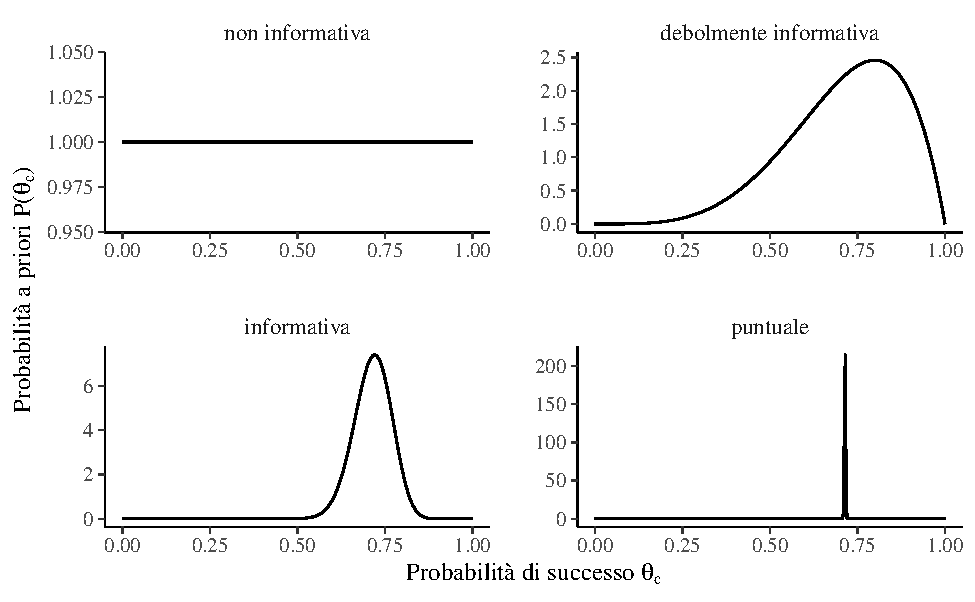
\includegraphics{ds4psy_files/figure-latex/ch-03-02-models-types-of-priors-1} 

}

\caption{Esempi di distribuzioni a priori per il parametro $\theta_c$ nel Modello Binomiale.}\label{fig:ch-03-02-models-types-of-priors}
\end{figure}

\hypertarget{selezione-della-distribuzione-a-priori}{%
\subsection{Selezione della distribuzione a priori}\label{selezione-della-distribuzione-a-priori}}

La selezione delle distribuzioni a priori è stata spesso vista come una delle scelte più importanti che un ricercatore fa quando implementa un modello bayesiano in quanto può avere un impatto sostanziale sui risultati finali. La soggettività delle distribuzioni a priori è evidenziata dai critici come un potenziale svantaggio dei metodi bayesiani. A questa critica, \citet{vandeSchoot2021modelling} rispondono dicendo che, al di là della scelta delle distribuzioni a priori, ci sono molti elementi del processo di inferenza statistica che sono soggettivi, ovvero la scelta del modello statistico e le ipotesi sulla distribuzione degli errori. In secondo luogo, \citet{vandeSchoot2021modelling} notano come le distribuzioni a priori svolgono due importanti ruoli statistici: quello della ``regolarizzazione della stima'', ovvero, il processo che porta ad indebolire l'influenza indebita di osservazioni estreme, e quello del miglioramento dell'efficienza della stima, ovvero, la facilitazione dei processi di calcolo numerico di stima della distribuzione a posteriori. L'effetto della distribuzione a priori sulla distribuzione a posteriori verrà discusso nel Capitolo \ref{chapter-balance}.

\hypertarget{la-distribuzione-a-priori-per-i-dati-di-zetschefuture2019}{%
\subsection{\texorpdfstring{La distribuzione a priori per i dati di \citet{zetschefuture2019}}{La distribuzione a priori per i dati di @zetschefuture2019}}\label{la-distribuzione-a-priori-per-i-dati-di-zetschefuture2019}}

In un problema concreto di analisi dei dati, la scelta della distribuzione a priori dipende dalle credenze a priori che vogliamo includere nell'analisi dei dati. Se non abbiamo alcuna informazione a priori, potremmo pensare di usare una distribuzione a priori uniforme, ovvero una Beta di parametri \(\alpha=1\) e \(\beta=1\). Questa, tuttavia, è una cattiva idea perché il risultato ottenuto non è invariante a seconda della trasformazione della scala dei dati (ad esempio, se esprimiamo l'altezza in cm piuttosto che in m). Il problema della \emph{riparametrizzazione} verrà discusso nel Capitolo ?? \textbf{TODO}. È invece raccomandato usare una distribuzione a priori poco informativa, come ad esempio \(\mbox{Beta}(2, 2)\).

Nella presente discussione, per fare un esempio, quale distribuzione a priori useremo una \(\mbox{Beta}(2, 10)\), ovvero:

\[
p(\theta) = \frac{\Gamma(12)}{\Gamma(2)\Gamma(10)}\theta^{2-1} (1-\theta)^{10-1}.
\]

\begin{Shaded}
\begin{Highlighting}[]
\NormalTok{bayesrules}\SpecialCharTok{::}\FunctionTok{plot\_beta}\NormalTok{(}\AttributeTok{alpha =} \DecValTok{2}\NormalTok{, }\AttributeTok{beta =} \DecValTok{10}\NormalTok{, }\AttributeTok{mean =} \ConstantTok{TRUE}\NormalTok{, }\AttributeTok{mode =} \ConstantTok{TRUE}\NormalTok{)}
\end{Highlighting}
\end{Shaded}

\begin{center}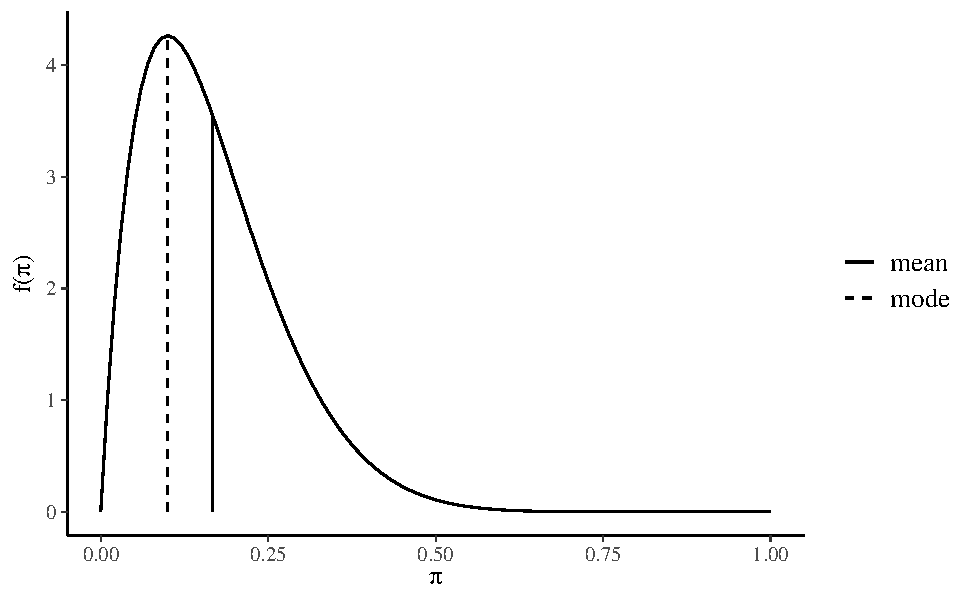
\includegraphics{ds4psy_files/figure-latex/unnamed-chunk-2-1} \end{center}

\noindent La \(\mbox{Beta}(2, 10)\) esprime la credenza che \(\theta\) assume valori \(< 0.5\), con il valore più plausibile pari a circa 0.1. Questo è assolutamente implausibile, nel caso dell'esempio in discussione. Adotteremo una tale distribuzione a priori solo per scopi didattici, per esplorare le conseguenze di tale scelta (molto più sensato sarebbe stato usare \(\mbox{Beta}(2, 2)\)).

\hypertarget{verosimiglianza}{%
\section{Verosimiglianza}\label{verosimiglianza}}

Oltre alla distribuzione a priori di \(\theta\), nel numeratore della regola di Bayes troviamo la funzione di verosimigliana. Iniziamo dunque con una definizione.

\begin{definition}
La \emph{funzione di verosimiglianza} \(\mathcal{L}(\theta \mid y) = f(y \mid \theta), \theta \in \Theta,\) è la funzione di massa o di densità di probabilità dei dati \(y\) vista come una funzione del parametro sconosciuto (o dei parametri sconosciuti) \(\theta\).
\end{definition}

Detto in altre parole, le funzioni di verosimiglianza e di (massa o densità di) probabilità sono formalmente identiche, ma è completamente diversa la loro interpretazione. Nel caso della funzione di massa o di densità di probabilità la distribuzione del vettore casuale delle osservazioni campionarie \(y\) dipende dai valori assunti dal parametro (o dai parametri) \(\theta\); nel caso della la funzione di verosimiglianza la credibilità assegnata a ciascun possibile valore \(\theta\) viene determinata avendo acquisita l'informazione campionaria \(y\) che rappresenta l'elemento condizionante. In altri termini, la funzione di verosimiglianza è lo strumento che consente di rispondere alla seguente domanda: avendo osservato i dati \(y\), quanto risultano (relativamente) credibili i diversi valori del parametro \(\theta\)?

Spesso per indicare la verosimiglianza si scrive \(\mathcal{L}(\theta)\) se è chiaro a quali valori \(y\) ci si riferisce. La verosimiglianza \(\mathcal{L}\) è una curva (in generale, una superficie) nello spazio \(\Theta\) del parametro (in generale, dei parametri) che riflette la credibilità relativa dei valori \(\theta\) alla luce dei dati osservati.

Notiamo un punto importante: la funzione \(\mathcal{L}(\theta \mid y)\) non è una funzione di densità. Infatti, essa non racchiude un'area unitaria.

In conclusione, la funzione di verosimiglianza descrive in termini relativi il sostegno empirico che \(\theta \in \Theta\) riceve da \(y\). Infatti, la funzione di verosimiglianza assume forme diverse al variare di \(y\) (lasciamo come esercizio da svolgere la verifica di questa affermazione).

\hypertarget{la-stima-di-massima-verosimiglianza}{%
\subsection{La stima di massima verosimiglianza}\label{la-stima-di-massima-verosimiglianza}}

La funzione di verosimiglianza rappresenta la ``credibilità relativa'' dei valori del parametro di interesse. Ma qual è il valore più credibile? Se utilizziamo soltanto la funzione di verosimiglianza, allora la risposta è data dalla stima di massima verosimiglinza.

\begin{definition}
Un valore di \(\theta\) che massimizza \(\mathcal{L}(\theta \mid y)\) sullo spazio parametrico \(\Theta\) è detto \emph{stima di massima verosimiglinza} (s.m.v.) di \(\theta\) ed è indicato con \(\hat{\theta}\):

\begin{equation}
\hat{\theta} = \argmax_{\theta \in \Theta} \mathcal{L}(\theta).
\end{equation}
\end{definition}

Il paradigma frequentista utilizza la funzione di verosimiglianza quale unico strumento per giungere alla stima del valore più credibile del parametro sconosciuto \(\theta\). Tale stima corrisponde al punto di massimo della funzione di verosimiglianza. In base all'approccio bayesiano, invece, il valore più credibile del parametro sconosciuto \(\theta\), anziché alla s.m.v., corrisponde invece alla moda (o media, o mediana) della distribuzione a posteriori \(p(\theta \mid y)\) che si ottiene combinando la verosimiglianza \(p(y \mid \theta)\) con la distribuzione a priori \(p(\theta)\). Per un approfondimento della stima di massima verosimiglianza si veda l'Appendice \ref{appendix:max-like}.

\hypertarget{la-log-verosimiglianza}{%
\subsection{La log-verosimiglianza}\label{la-log-verosimiglianza}}

Dal punto di vista pratico risulta più conveniente utilizzare, al posto della funzione di verosimiglianza, il suo logaritmo naturale, ovvero la funzione di log-verosimiglianza:

\begin{equation}
\ell(\theta) = \log \mathcal{L}(\theta).
\end{equation}

Poiché il logaritmo è una funzione strettamente crescente (usualmente si considera il logaritmo naturale), allora \(\mathcal{L}(\theta)\) e \(\ell(\theta)\) assumono il massimo (o i punti di massimo) in corrispondenza degli stessi valori di \(\theta\):

\[
\hat{\theta} = \argmax_{\theta \in \Theta} \ell(\theta) = \argmax_{\theta \in \Theta} \mathcal{L}(\theta).
\]

Per le proprietà del logaritmo, si ha

\begin{equation}
\ell(\theta) = \log \left( \prod_{i = 1}^n f(y \mid \theta) \right) = \sum_{i = 1}^n \log f(y \mid \theta).
\end{equation}

Si noti che non è necessario lavorare con i logaritmi, ma è fortemente consigliato. Il motivo è che i valori della verosimiglianza, in cui si moltiplicano valori di probabilità molto piccoli, possono diventare estremamente piccoli -- qualcosa come \(10^{-34}\). In tali circostanze, non è sorprendente che i programmi dei computer mostrino problemi di arrotondamento numerico. Le trasformazioni logaritmiche risolvono questo problema.

\begin{remark}
Seguendo una pratica comune, in questa dispensa spesso useremo la notazione \(p(\cdot)\) per rappresentare due quantità differenti, ovvero la funzione di verosimiglianza e la distribuzione a priori. Questo piccolo abuso di notazione riflette il seguente punto di vista: anche se la verosimiglianza non è una funzione di densità di probabilità, noi non vogliamo stressare questo aspetto, ma vogliamo piuttosto pensare alla verosimiglianza e alla distribuzione a priori come a due elementi che sono egualmente necessari per calcolare la distribuzione a posteriori. In altri termini, per così dire, questa notazione assegna lo stesso status epistemologico alle due diverse quantità che si trovano al numeratore della regola di Bayes.
\end{remark}

\begin{exercise}
Per i dati di \citet{zetschefuture2019}, ovvero 23 ``successi'' in 30 prove, si trovi e si interpreti la funzione di verosimiglianza.
\end{exercise}

Per i dati di \citet{zetschefuture2019} la funzione di verosimiglianza corrisponde alla funzione binomiale di parametro \(\theta \in [0, 1]\) sconosciuto. Abbiamo osservato un ``successo'' 23 volte in 30 ``prove'', dunque, \(y = 23\) e \(n = 30\). La funzione di verosimiglianza diventa

\begin{equation}
\mathcal{L}(\theta \mid y) = \frac{(23 + 7)!}{23!7!} \theta^{23} + (1-\theta)^7.
\label{eq:likebino23}
\end{equation}

Per costruire la funzione di verosimiglianza dobbiamo applicare la \eqref{eq:likebino23} tante volte, cambiando ogni volta il valore \(\theta\) ma \emph{tenendo sempre costante il valore dei dati}. Per esempio, se poniamo \(\theta = 0.1\)

\[
\mathcal{L}(\theta \mid y) = \frac{(23 + 7)!}{23!7!} 0.1^{23} + (1-0.1)^7
\]

otteniamo

\begin{Shaded}
\begin{Highlighting}[]
\FunctionTok{dbinom}\NormalTok{(}\DecValTok{23}\NormalTok{, }\DecValTok{30}\NormalTok{, }\FloatTok{0.1}\NormalTok{)}
\CommentTok{\#\textgreater{} [1] 9.737e{-}18}
\end{Highlighting}
\end{Shaded}

Se poniamo \(\theta = 0.2\)

\[
\mathcal{L}(\theta \mid y) = \frac{(23 + 7)!}{23!7!} 0.2^{23} + (1-0.2)^7
\]

otteniamo

\begin{Shaded}
\begin{Highlighting}[]
\FunctionTok{dbinom}\NormalTok{(}\DecValTok{23}\NormalTok{, }\DecValTok{30}\NormalTok{, }\FloatTok{0.2}\NormalTok{)}
\CommentTok{\#\textgreater{} [1] 3.581e{-}11}
\end{Highlighting}
\end{Shaded}

e così via. La figura \ref{fig:likefutexpect} --- costruita utilizzando 100 valori equispaziati \(\theta \in [0, 1]\) --- fornisce una rappresentazione grafica della funzione di verosimiglianza.

\begin{Shaded}
\begin{Highlighting}[]
\NormalTok{n }\OtherTok{\textless{}{-}} \DecValTok{30}
\NormalTok{y }\OtherTok{\textless{}{-}} \DecValTok{23}
\NormalTok{theta }\OtherTok{\textless{}{-}} \FunctionTok{seq}\NormalTok{(}\DecValTok{0}\NormalTok{, }\DecValTok{1}\NormalTok{, }\AttributeTok{length.out =} \DecValTok{100}\NormalTok{)}
\NormalTok{like }\OtherTok{\textless{}{-}} \FunctionTok{choose}\NormalTok{(n, y) }\SpecialCharTok{*}\NormalTok{ theta}\SpecialCharTok{\^{}}\NormalTok{y }\SpecialCharTok{*}\NormalTok{ (}\DecValTok{1} \SpecialCharTok{{-}}\NormalTok{ theta)}\SpecialCharTok{\^{}}\NormalTok{(n }\SpecialCharTok{{-}}\NormalTok{ y)}
\FunctionTok{tibble}\NormalTok{(theta, like) }\SpecialCharTok{\%\textgreater{}\%}
  \FunctionTok{ggplot}\NormalTok{(}\FunctionTok{aes}\NormalTok{(}\AttributeTok{x =}\NormalTok{ theta, }\AttributeTok{y =}\NormalTok{ like)) }\SpecialCharTok{+}
  \FunctionTok{geom\_line}\NormalTok{() }\SpecialCharTok{+}
  \FunctionTok{labs}\NormalTok{(}
    \AttributeTok{y =} \FunctionTok{expression}\NormalTok{(}\FunctionTok{L}\NormalTok{(theta)),}
    \AttributeTok{x =} \FunctionTok{expression}\NormalTok{(}\StringTok{"Valori possibili di"} \SpecialCharTok{\textasciitilde{}}\NormalTok{ theta)}
\NormalTok{  )}
\end{Highlighting}
\end{Shaded}

\begin{figure}[h]

{\centering 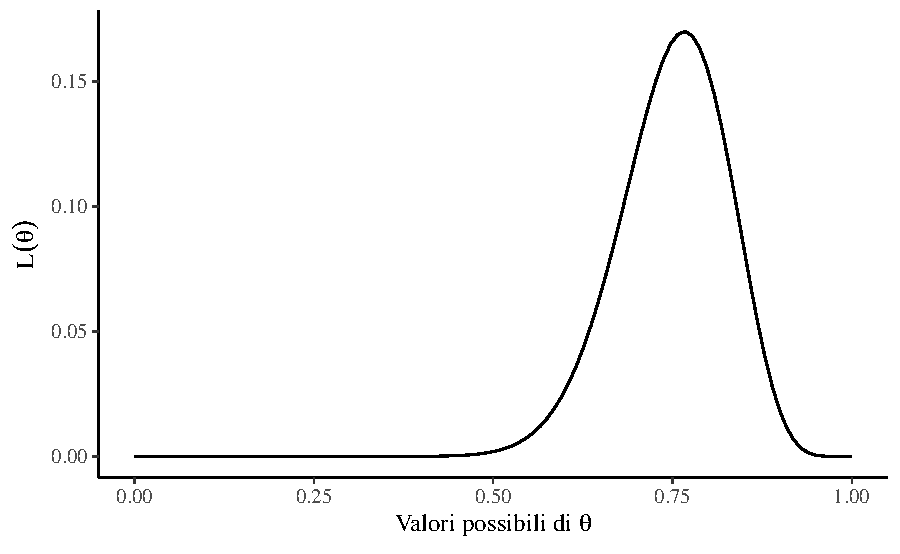
\includegraphics{ds4psy_files/figure-latex/likefutexpect-1} 

}

\caption{Funzione di verosimiglianza nel caso di 23 successi in 30 prove.}\label{fig:likefutexpect}
\end{figure}

Come possiamo interpretare la curva che abbiamo ottenuto? Per alcuni valori \(\theta\) la funzione di verosimiglianza assume valori piccoli; per altri valori \(\theta\) la funzione di verosimiglianza assume valori più grandi. Questi ultimi sono i valori di \(\theta\) ``più credibili'' e il valore 23/30 è il valore più credibile di tutti. La funzione di verosimiglianza di \(\theta\) valuta la compatibilità dei dati osservati \(Y = y\) con i diversi possibili valori \(\theta\). In termini più formali possiamo dire che la funzione di verosimiglianza ha la seguente interpretazione: sulla base dei dati, \(\theta_1 \in \Theta\) è più credibile di \(\theta_2 \in \Theta\) come indice del modello probabilistico generatore delle osservazioni se \(\mathcal{L}(\theta_1) > \mathcal{L}(\theta_1)\).

\hypertarget{sec:const-normaliz-bino23}{%
\section{La verosimiglianza marginale}\label{sec:const-normaliz-bino23}}

Per il calcolo di \(p(\theta \mid y)\) è necessario dividere il prodotto tra la distribuzione a priori e la verosimiglianza per una costante di normalizzazione. Tale costante di normalizzazione, detta \emph{verosimiglianza marginale}, ha lo scopo di fare in modo che \(p(\theta \mid y)\) abbia area unitaria.

Si noti che il denominatore della regola di Bayes (ovvero la verosimiglianza marginale) è sempre espresso nei termini di un integrale. Tranne in pochi casi particolari, tale integrale non ha una soluzione analitica. Per questa ragione, l'inferenza bayesiana procede calcolando una approssimazione della distribuzione a posteriori mediante metodi numerici.

\begin{exercise}
Si trovi la verosimiglianza maginale per i dati di \citet{zetschefuture2019}.

Supponiamo che nel numeratore bayesiano la verosimiglianza sia moltiplicata per una distribuzione uniforme, \(\mbox{Beta}(1, 1)\). In questo caso, il prodotto si riduce alla funzione di verosimiglianza. In riferimento ai dati di \citet{zetschefuture2019}, la costante di normalizzazione per si ottiene semplicemente marginalizzando la funzione di verosimiglianza \(p(y = 23, n = 30 \mid \theta)\) sopra \(\theta\), ovvero risolvendo l'integrale:

\begin{equation}
p(y = 23, n = 30) = \int_0^1 \binom{30}{23} \theta^{23} (1-\theta)^{7} \,\operatorname {d}\!\theta.
\label{eq:intlikebino23}
\end{equation}

Una soluzione numerica si trova facilmente usando \(\R\):

\begin{Shaded}
\begin{Highlighting}[]
\NormalTok{like\_bin }\OtherTok{\textless{}{-}} \ControlFlowTok{function}\NormalTok{(theta) \{}
  \FunctionTok{choose}\NormalTok{(}\DecValTok{30}\NormalTok{, }\DecValTok{23}\NormalTok{) }\SpecialCharTok{*}\NormalTok{ theta}\SpecialCharTok{\^{}}\DecValTok{23} \SpecialCharTok{*}\NormalTok{ (}\DecValTok{1} \SpecialCharTok{{-}}\NormalTok{ theta)}\SpecialCharTok{\^{}}\DecValTok{7}
\NormalTok{\}}
\FunctionTok{integrate}\NormalTok{(like\_bin, }\AttributeTok{lower =} \DecValTok{0}\NormalTok{, }\AttributeTok{upper =} \DecValTok{1}\NormalTok{)}\SpecialCharTok{$}\NormalTok{value}
\CommentTok{\#\textgreater{} [1] 0.03226}
\end{Highlighting}
\end{Shaded}

La derivazione analitica della costante di normalizzazione qui discussa è fornita nell'Appendice \ref{appendix:const-norm-bino23}.
\end{exercise}

\hypertarget{distribuzione-a-posteriori}{%
\section{Distribuzione a posteriori}\label{distribuzione-a-posteriori}}

La distribuzione a postreriori si trova applicando il teorema di Bayes:

\[
\text{probabilità a posteriori} = \frac{\text{probabilità a priori} \cdot \text{verosimiglianza}}{\text{costante di normalizzazione}}
\]

Ci sono due metodi principali per calcolare la distribuzione a posteriori \(p(\theta \mid y)\):

\begin{itemize}
\item
  una precisa derivazione matematica formulata nei termini della distribuzione a priori coniugata alla distribuzione a posteriori (si veda il Capitolo \ref{chapter-distr-coniugate}); tale procedura però ha un'applicabilità molto limitata;
\item
  un metodo approssimato, molto facile da utilizzare in pratica, che dipende da metodi Monte Carlo basati su Catena di Markov (MCMC); questo problema verrà discusso nel Capitolo ??
\end{itemize}

Una volta trovata la distribuzione a posteriori, possiamo usarla per derivare altre quantità di interesse. Questo viene generalmente ottenuto calcolando il valore atteso:

\[
J = \int f(\theta) p(\theta \mid y) \,\operatorname {d}\!y
\]

Se \(f(\cdot)\) è la funzione identità, ad esempio, \(J\) risulta essere la media di \(\theta\):

\[
\bar{\theta} = \int_{\Theta} \theta p(\theta \mid y) \,\operatorname {d}\!\theta .
\]

\hypertarget{distribuzione-predittiva-a-priori}{%
\section{Distribuzione predittiva a priori}\label{distribuzione-predittiva-a-priori}}

La distribuzione a posteriori è l'oggetto centrale nella statistica bayesiana, ma non è l'unico. Oltre a fare inferenze sui valori dei parametri, potremmo voler fare inferenze sui dati. Questo può essere fatto calcolando la \emph{distribuzione predittiva a priori}:

\begin{equation}
p(y^*) = \int_\Theta p(y^* \mid \theta) p(\theta) \,\operatorname {d}\!\theta .
\label{eq:prior-pred-distr}
\end{equation}

La \eqref{eq:prior-pred-distr} descrive la distribuzione prevista dei dati in base al modello (che include la distribuzione a priori e la verosimiglianza). Questi sono i dati \(y^*\) che ci aspettiamo, dato il modello, prima di avere osservato i dati del campione.

Possiamo utilizzare campioni dalla distribuzione predittiva a priori per valutare e calibrare i modelli utilizzando le nostre conoscenze dominio-specifiche. Ad esempio, ci potremmo chiedere: ``È sensato che un modello dell'altezza umana preveda che un essere umano sia alto -1.5 metri?''. Già prima di misurare una singola persona, possiamo renderci conto dell'assurdità di questa domanda. Se la distribuzione prevista dei dati consente domande di questo tipo, è chiaro che il modello deve essere riformulato.

\begin{remark}
Si dice comunemente che l'adozione di una prospettiva probabilistica per la modellazione conduce all'idea che i modelli generano dati. Se i modelli generano dati, possiamo creare modelli adatti per i nostri dati solo pensando a come i dati potrebbero essere stati generati. Inoltre, questa idea non è solo un concetto astratto. Assume una concreta nella forma della distribuzione predittiva a priori. Se la distribuzione predittiva a priori non ha senso, come abbiamo detto sopra, diventa necessario riformulare il modello.
\end{remark}

\hypertarget{distribuzione-predittiva-a-posteriori}{%
\section{Distribuzione predittiva a posteriori}\label{distribuzione-predittiva-a-posteriori}}

Un'altra quantità utile da calcolare è la distribuzione predittiva a posteriori:

\begin{equation}
p(\tilde{y} \mid y) = \int_\Theta p(\tilde{y} \mid \theta) p(\theta \mid y) \,\operatorname {d}\!\theta .
\label{eq:post-pred-distr}
\end{equation}

Questa è la distribuzione dei dati attesi futuri \(\tilde{y}\) alla luce della distribuzione a posteriori \(p(\theta \mid y)\), che a sua volta è una conseguenza del modello (distribuzione a priori e verosimiglianza) e dei dati osservati. In altre parole, questi sono i dati che il modello si aspetta dopo aver osservato i dati \(y\). Dalla \eqref{eq:post-pred-distr} possiamo vedere che le previsioni sui dati attesi futuri sono calcolate integrando (o marginalizzando) sulla distribuzione a posteriori dei parametri. Di conseguenza, le previsioni calcolate in questo modo incorporano l'incertezza relativa alla stima dei parametri del modello.

\hypertarget{commenti-e-considerazioni-finali}{%
\section*{Commenti e considerazioni finali}\label{commenti-e-considerazioni-finali}}


Questo Capitolo ha brevemente passato in rassegna alcuni concetti di base dell'inferenza statistica bayesiana. In base all'approccio bayesiano, invece di dire che il parametro di interesse di un modello statistico ha un valore vero ma sconosciuto, diciamo che, prima di eseguire l'esperimento, è possibile assegnare una distribuzione di probabilità, che chiamano stato di credenza, a quello che è il vero valore del parametro. Questa distribuzione a priori può essere nota (per esempio, sappiamo che la distribuzione dei punteggi del QI è normale con media 100 e deviazione standard 15) o può essere del tutto arbitraria. L'inferenza bayesiana procede poi nel modo seguente: si raccolgono alcuni dati e si calcola la probabilità dei possibili valori del parametro alla luce dei dati osservati e delle credenze a priori. Questa nuova distribuzione di probabilità è chiamata ``distribuzione a posteriori'' e riassume l'incertezza dell'inferenza. I concetti importanti che abbiamo appreso in questo Capitolo sono quelli di distribuzione a priori, verosimiglianza, verosimiglianza marginale e distribuzione a posteriori. Questi sono i concetti fondamentali della statistica bayesiana.

\hypertarget{metropolis}{%
\chapter{Approssimazione della distribuzione a posteriori}\label{metropolis}}

È possibile distinguere cinque metodi per il calcolo delle proprietà di una distribuzione.

\begin{enumerate}
\def\labelenumi{\arabic{enumi}.}
\tightlist
\item
  \textbf{Metodi analitici esatti:} per esempio, nel caso delle famiglie coniugate, quando disponiamo di una forma analitica della distribuzione a posteriori.
\item
  \textbf{Metodi numerici esatti:} dove, sebbene non sia disponibile alcuna formula algebrica in forma chiusa, le proprietà della distribuzione a posteriori possono essere calcolate con una precisione arbitraria -- vedremo un esempio di come questo possa essere fatto nella seguente discussione sui metodi basati su griglia.
\item
  \textbf{Metodi analitici approssimati:} per esempio, nel caso di approssimazioni normali alle distribuzioni di variabili casuali -- in questo Capitolo verrà discussa l'approssimazione quadratica della distribuzione a posteriori che è un esempio di questo approccio.
\item
  \textbf{Sperimentazione fisica:} ad esempio, quando un esperimento viene fisicamente ripetuto molte volte per determinare la proporzione empirica dei ``successi''.
\item
  \textbf{Simulazione al computer:} utilizzando appropriate funzioni di numeri casuali, viene generato un ampio campione di casi della variabile casuale per poi stimare empiricamente la proprietà di interesse in base al campione così otttenuto. Questa tecnica è conosciuta come metodo di Monte Carlo ed è il metodo che verrà utilizzato nella seconda parte di questa dispensa.
\end{enumerate}

In questo Capitolo verranno esaminate tre diverse tecniche che possono essere utilizzate per calcolare per via numerica la distribuzione a posteriori:

\begin{enumerate}
\def\labelenumi{\arabic{enumi}.}
\tightlist
\item
  il metodo basato su griglia;
\item
  il metodo dell'approssimazione quadratica,
\item
  il metodo basato su simulazione di Monte Carlo basato su Catena di Markov (MCMC).
\end{enumerate}

\hypertarget{metodo-basato-su-griglia}{%
\section{Metodo basato su griglia}\label{metodo-basato-su-griglia}}

Il metodo basato su griglia (\emph{grid-based}) è un metodo numerico esatto basato su una griglia di punti uniformemente spaziati. Anche se la maggior parte dei parametri è continua (ovvero, in linea di principio ciascun parametro può assumere un numero infinito di valori), possiamo ottenere un'eccellente approssimazione della distribuzione a posteriori considerando solo una griglia finita di valori dei parametri. In un tale metodo, la densità di probabilità a posteriori può dunque essere approssimata tramite le densità di probabilità calcolate in ciascuna cella della griglia.

Il metodo basato su griglia si sviluppa in quattro fasi:

\begin{itemize}
\tightlist
\item
  fissare una griglia discreta di possibili valori \(\theta\);\footnote{È chiaro che, per ottenere buone approssimazioni, è necessaria una griglia molto densa.}
\item
  valutare la distribuzione a priori \(p(\theta)\) e la funzione di verosimiglianza \(\mathcal{L}(y \mid \theta)\) in corrispondenza di ciascun valore \(\theta\) della griglia;
\item
  ottenere un'approssimazione discreta della densità a posteriori:

  \begin{itemize}
  \tightlist
  \item
    per ciascun valore \(\theta\) della griglia, calcolare il prodotto \(p(\theta) \mathcal{L} (y \mid \theta)\);
  \item
    normalizzare i prodotti così ottenuti in modo tale che la loro somma sia 1;
  \end{itemize}
\item
  selezionare \(N\) valori casuali della griglia in modo tale da ottenere un campione casuale delle densità a posteriori normalizzate.
\end{itemize}

Possiamo migliorare l'approssimazione aumentando il numero di punti della griglia. Infatti utilizzando un numero infinito di punti si otterrebbe la descrizione esatta della distribuzione a posteriori, dovendo però pagare il costo dell'utilizzo di infinite risorse di calcolo. Il limite maggiore dell'approccio basato su griglia è che al crescere della dimensionalità \(N\) dello spazio dei parametri i punti della griglia necessari per avere una buona stima crescerebbero esponenzialmente con \(N\), rendendo questo metodo inattuabile.

\hypertarget{modello-beta-binomiale}{%
\subsection{Modello Beta-Binomiale}\label{modello-beta-binomiale}}

Per fare un esempio, consideriamo il modello Beta-Binomiale di cui conosciamo la soluzione esatta. Supponiamo di avere osservato 9 sucessi in 10 prove Bernoulliane indipendenti.\footnote{La discussione del modello Beta-Binomiale segue molto da vicino la presentazione di \citet{Johnson2022bayesrules} utilizzando anche lo stesso codice \R.} Imponiamo alla distribuzione a priori su \(\theta\) (proabilità di successo in una singola prova) una Beta(2, 2) per descrivere la nostra incertezza sul parametro prima di avere osservato i dati. Dunque, il modello diventa:

\begin{align}
Y \mid \theta & \sim \text{Bin}(10, \pi) \notag\\
\theta & \sim \mbox{Beta}(2, 2).\notag
\end{align}

In queste circostanze, l'aggiornamento bayesiano produce una distribuzione a posteriori Beta di parametri 11 (\(y + \alpha\) = 9 + 2) e 3 (\(n - y + \beta\) = 10 - 9 + 2):

\begin{equation}
\theta \mid (y = 9) \sim \mbox{Beta}(11, 3).\notag
\end{equation}

Per approssimare la distribuzione a posteriori, fissiamo una griglia di \(n = 6\) valori equispaziati: \(\theta \in \{0, 0.2, 0.4, 0.6, 0.8, 1\}\) (in seguito aumenteremo \(n\)):

\begin{Shaded}
\begin{Highlighting}[]
\NormalTok{grid\_data }\OtherTok{\textless{}{-}} \FunctionTok{tibble}\NormalTok{(}
  \AttributeTok{theta\_grid =} \FunctionTok{seq}\NormalTok{(}\AttributeTok{from =} \DecValTok{0}\NormalTok{, }\AttributeTok{to =} \DecValTok{1}\NormalTok{, }\AttributeTok{length =} \DecValTok{6}\NormalTok{)}
\NormalTok{)}
\end{Highlighting}
\end{Shaded}

In corrispondenza di ciascun valore della griglia, valutiamo la distribuzione a priori \(\mbox{Beta}(2, 2)\) e la verosimiglianza \(\Bin(10, \theta)\) con \(y = 9\).

\begin{Shaded}
\begin{Highlighting}[]
\NormalTok{grid\_data }\OtherTok{\textless{}{-}}\NormalTok{ grid\_data }\SpecialCharTok{\%\textgreater{}\%}
  \FunctionTok{mutate}\NormalTok{(}
    \AttributeTok{prior =} \FunctionTok{dbeta}\NormalTok{(theta\_grid, }\DecValTok{2}\NormalTok{, }\DecValTok{2}\NormalTok{),}
    \AttributeTok{likelihood =} \FunctionTok{dbinom}\NormalTok{(}\DecValTok{9}\NormalTok{, }\DecValTok{10}\NormalTok{, theta\_grid)}
\NormalTok{  )}
\end{Highlighting}
\end{Shaded}

In ciascuna cella della griglia calcoliamo poi il prodotto della verosimiglianza e della distribuzione a priori. Troviamo così un'approssimazione discreta e non normalizzata della distribuzione a posteriori (\texttt{unnormalized}). Normalizziamo infine questa approssimazione dividendo ciascun valore del vettore \texttt{unnormalized} per la somma di tutti i valori del vettore:

\begin{Shaded}
\begin{Highlighting}[]
\NormalTok{grid\_data }\OtherTok{\textless{}{-}}\NormalTok{ grid\_data }\SpecialCharTok{\%\textgreater{}\%}
  \FunctionTok{mutate}\NormalTok{(}
    \AttributeTok{unnormalized =}\NormalTok{ likelihood }\SpecialCharTok{*}\NormalTok{ prior,}
    \AttributeTok{posterior =}\NormalTok{ unnormalized }\SpecialCharTok{/} \FunctionTok{sum}\NormalTok{(unnormalized)}
\NormalTok{  )}
\end{Highlighting}
\end{Shaded}

La somma dei valori così trovati sarà uguale a 1:

\begin{Shaded}
\begin{Highlighting}[]
\NormalTok{grid\_data }\SpecialCharTok{\%\textgreater{}\%}
  \FunctionTok{summarize}\NormalTok{(}
    \FunctionTok{sum}\NormalTok{(unnormalized),}
    \FunctionTok{sum}\NormalTok{(posterior)}
\NormalTok{  )}
\CommentTok{\#\textgreater{} \# A tibble: 1 x 2}
\CommentTok{\#\textgreater{}   \textasciigrave{}sum(unnormalized)\textasciigrave{} \textasciigrave{}sum(posterior)\textasciigrave{}}
\CommentTok{\#\textgreater{}                 \textless{}dbl\textgreater{}            \textless{}dbl\textgreater{}}
\CommentTok{\#\textgreater{} 1               0.318                1}
\end{Highlighting}
\end{Shaded}

Abbiamo dunque ottenuto la seguente distribuzione a posteriori discretizzata \(p(\theta \mid y)\):

\begin{Shaded}
\begin{Highlighting}[]
\FunctionTok{round}\NormalTok{(grid\_data, }\DecValTok{2}\NormalTok{)}
\CommentTok{\#\textgreater{} \# A tibble: 6 x 5}
\CommentTok{\#\textgreater{}   theta\_grid prior likelihood unnormalized posterior}
\CommentTok{\#\textgreater{}        \textless{}dbl\textgreater{} \textless{}dbl\textgreater{}      \textless{}dbl\textgreater{}        \textless{}dbl\textgreater{}     \textless{}dbl\textgreater{}}
\CommentTok{\#\textgreater{} 1        0    0          0            0         0   }
\CommentTok{\#\textgreater{} 2        0.2  0.96       0            0         0   }
\CommentTok{\#\textgreater{} 3        0.4  1.44       0            0         0.01}
\CommentTok{\#\textgreater{} 4        0.6  1.44       0.04         0.06      0.18}
\CommentTok{\#\textgreater{} 5        0.8  0.96       0.27         0.26      0.81}
\CommentTok{\#\textgreater{} 6        1    0          0            0         0}
\end{Highlighting}
\end{Shaded}

La figura \ref{fig:grid-method-6points-posterior-plot} mostra un grafico della distribuzione a posteriori discretizzata che è stata ottenuta:

\begin{Shaded}
\begin{Highlighting}[]
\NormalTok{grid\_data }\SpecialCharTok{\%\textgreater{}\%} 
  \FunctionTok{ggplot}\NormalTok{(}
    \FunctionTok{aes}\NormalTok{(}\AttributeTok{x =}\NormalTok{ theta\_grid, }\AttributeTok{y =}\NormalTok{ posterior)}
\NormalTok{  ) }\SpecialCharTok{+}
  \FunctionTok{geom\_point}\NormalTok{() }\SpecialCharTok{+}
  \FunctionTok{geom\_segment}\NormalTok{(}
    \FunctionTok{aes}\NormalTok{(}
      \AttributeTok{x =}\NormalTok{ theta\_grid, }
      \AttributeTok{xend =}\NormalTok{ theta\_grid, }
      \AttributeTok{y =} \DecValTok{0}\NormalTok{, }
      \AttributeTok{yend =}\NormalTok{ posterior)}
\NormalTok{  )}
\end{Highlighting}
\end{Shaded}

\begin{figure}[h]

{\centering 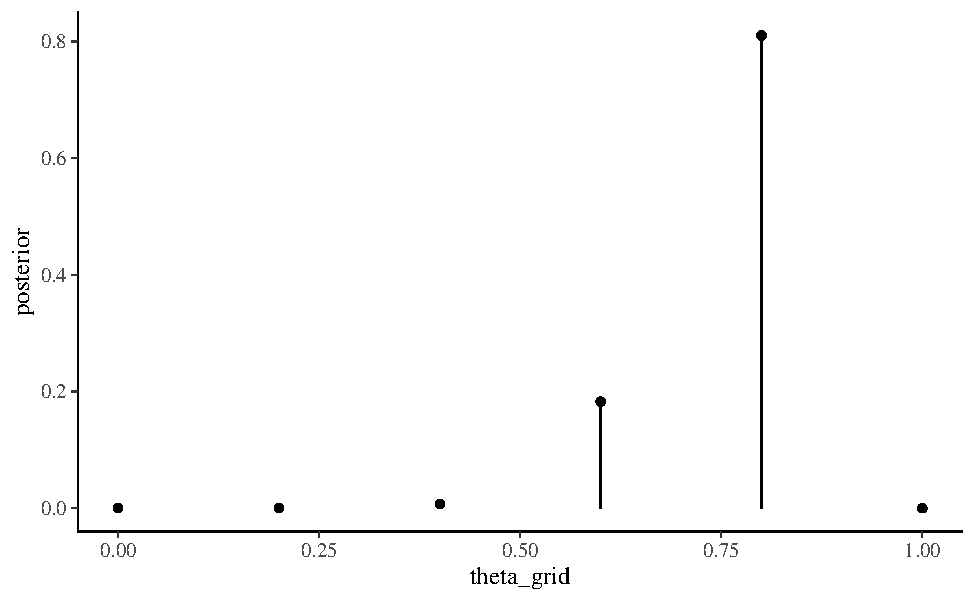
\includegraphics{ds4psy_files/figure-latex/grid-method-6points-posterior-plot-1} 

}

\caption{Distribuzione a posteriori discretizzata ottenuta con il metodo grid-based per $y$ = 9 successi in 10 prove Bernoulliane, con distribuzione a priori $\mbox{Beta}(2, 2)$. È stata utilizzata una griglia di solo $n$ = 6 punti.}\label{fig:grid-method-6points-posterior-plot}
\end{figure}

L'ultimo passo della simulazione è il campionamento dalla distribuzione a posteriori discretizzata:

\begin{Shaded}
\begin{Highlighting}[]
\FunctionTok{set.seed}\NormalTok{(}\DecValTok{84735}\NormalTok{)}
\NormalTok{post\_sample }\OtherTok{\textless{}{-}} \FunctionTok{sample\_n}\NormalTok{(}
\NormalTok{  grid\_data,}
  \AttributeTok{size =} \FloatTok{1e5}\NormalTok{,}
  \AttributeTok{weight =}\NormalTok{ posterior,}
  \AttributeTok{replace =} \ConstantTok{TRUE}
\NormalTok{)}
\end{Highlighting}
\end{Shaded}

È facile intuire che i valori estratti con rimessa dalla distribuzione a posteriori discretizzata saranno quasi sempre uguali a 0.6 o 0.8. Questa intuizione è confermata dal grafico \ref{fig:grid-method-6points-posterior-plot-sampling} a cui è stata sovrapposta la vera distribuzione a posteriori \(\mbox{Beta}(11, 3)\):

\begin{Shaded}
\begin{Highlighting}[]
\FunctionTok{ggplot}\NormalTok{(post\_sample, }\FunctionTok{aes}\NormalTok{(}\AttributeTok{x =}\NormalTok{ theta\_grid)) }\SpecialCharTok{+}
  \FunctionTok{geom\_histogram}\NormalTok{(}\FunctionTok{aes}\NormalTok{(}\AttributeTok{y =}\NormalTok{ ..density..), }\AttributeTok{color =} \StringTok{"white"}\NormalTok{) }\SpecialCharTok{+}
  \FunctionTok{stat\_function}\NormalTok{(}\AttributeTok{fun =}\NormalTok{ dbeta, }\AttributeTok{args =} \FunctionTok{list}\NormalTok{(}\DecValTok{11}\NormalTok{, }\DecValTok{3}\NormalTok{)) }\SpecialCharTok{+}
  \FunctionTok{lims}\NormalTok{(}\AttributeTok{x =} \FunctionTok{c}\NormalTok{(}\DecValTok{0}\NormalTok{, }\DecValTok{1}\NormalTok{))}
\end{Highlighting}
\end{Shaded}

\begin{figure}[h]

{\centering 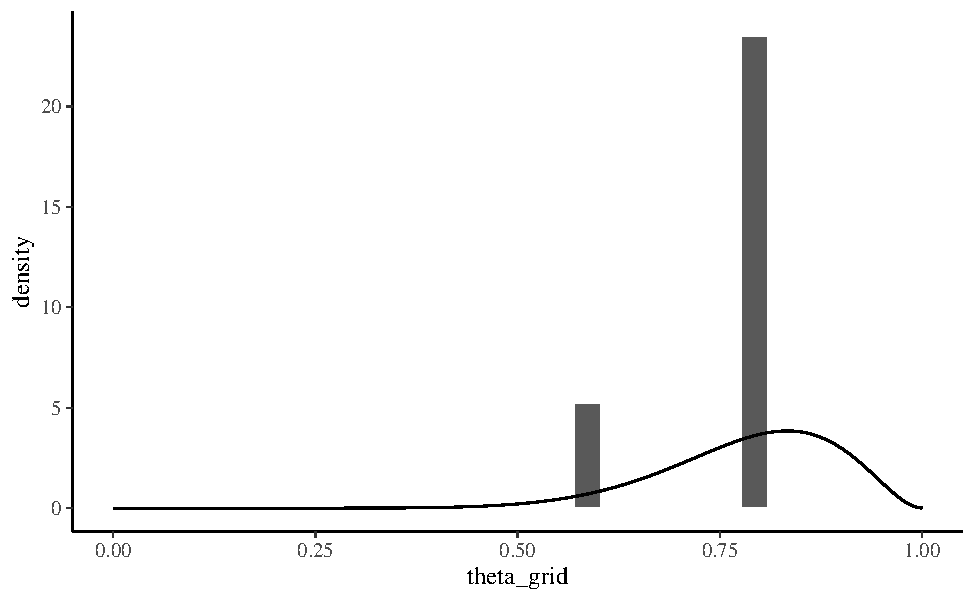
\includegraphics{ds4psy_files/figure-latex/grid-method-6points-posterior-plot-sampling-1} 

}

\caption{Campionamento dalla  distribuzione a posteriori discretizzata ottenuta con il metodo grid-based per $y$ = 9 successi in 10 prove Bernoulliane, con distribuzione a priori $\mbox{Beta}(2, 2)$. È stata utilizzata una griglia di solo $n$ = 6 punti.}\label{fig:grid-method-6points-posterior-plot-sampling}
\end{figure}

La figura \ref{fig:grid-method-6points-posterior-plot-sampling} mostra che, con una griglia così sparsa abbiamo ottenuto una versione estremamente approssimata della vera distribuzione a posteriori. Possiamo però ottenere un risultato migliore con una griglia più fine, come indicato dalla figura \ref{fig:grid-method-100points-posterior-plot-sampling}:

\begin{Shaded}
\begin{Highlighting}[]
\NormalTok{grid\_data }\OtherTok{\textless{}{-}} \FunctionTok{tibble}\NormalTok{(}
  \AttributeTok{theta\_grid =} \FunctionTok{seq}\NormalTok{(}\AttributeTok{from =} \DecValTok{0}\NormalTok{, }\AttributeTok{to =} \DecValTok{1}\NormalTok{, }\AttributeTok{length.out =} \DecValTok{100}\NormalTok{)}
\NormalTok{)}
\NormalTok{grid\_data }\OtherTok{\textless{}{-}}\NormalTok{ grid\_data }\SpecialCharTok{\%\textgreater{}\%}
  \FunctionTok{mutate}\NormalTok{(}
    \AttributeTok{prior =} \FunctionTok{dbeta}\NormalTok{(theta\_grid, }\DecValTok{2}\NormalTok{, }\DecValTok{2}\NormalTok{),}
    \AttributeTok{likelihood =} \FunctionTok{dbinom}\NormalTok{(}\DecValTok{9}\NormalTok{, }\DecValTok{10}\NormalTok{, theta\_grid)}
\NormalTok{  )}
\NormalTok{grid\_data }\OtherTok{\textless{}{-}}\NormalTok{ grid\_data }\SpecialCharTok{\%\textgreater{}\%}
  \FunctionTok{mutate}\NormalTok{(}
    \AttributeTok{unnormalized =}\NormalTok{ likelihood }\SpecialCharTok{*}\NormalTok{ prior,}
    \AttributeTok{posterior =}\NormalTok{ unnormalized }\SpecialCharTok{/} \FunctionTok{sum}\NormalTok{(unnormalized)}
\NormalTok{  )}
\NormalTok{grid\_data }\SpecialCharTok{\%\textgreater{}\%}
  \FunctionTok{ggplot}\NormalTok{(}
    \FunctionTok{aes}\NormalTok{(}\AttributeTok{x =}\NormalTok{ theta\_grid, }\AttributeTok{y =}\NormalTok{ posterior)}
\NormalTok{  ) }\SpecialCharTok{+}
  \FunctionTok{geom\_point}\NormalTok{() }\SpecialCharTok{+}
  \FunctionTok{geom\_segment}\NormalTok{(}
    \FunctionTok{aes}\NormalTok{(}
      \AttributeTok{x =}\NormalTok{ theta\_grid,}
      \AttributeTok{xend =}\NormalTok{ theta\_grid,}
      \AttributeTok{y =} \DecValTok{0}\NormalTok{,}
      \AttributeTok{yend =}\NormalTok{ posterior}
\NormalTok{    )}
\NormalTok{  )}
\end{Highlighting}
\end{Shaded}

\begin{figure}[h]

{\centering 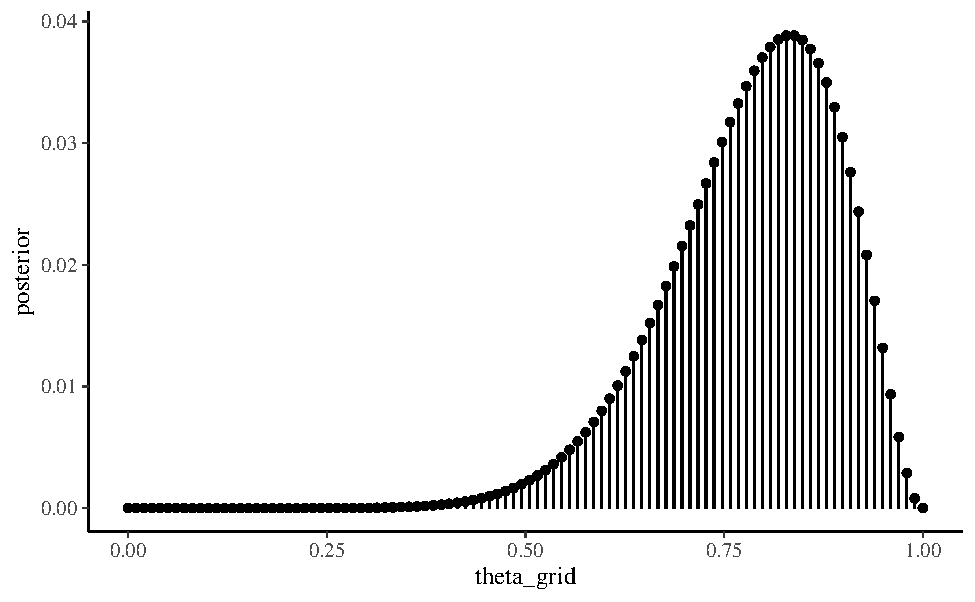
\includegraphics{ds4psy_files/figure-latex/grid-method-100points-posterior-plot-sampling-1} 

}

\caption{Distribuzione a posteriori discretizzata ottenuta con il metodo grid-based per $y$ = 9 successi in 10 prove Bernoulliane, con distribuzione a priori $\mbox{Beta}(2, 2)$. È stata utilizzata una griglia di $n$ = 100 punti.}\label{fig:grid-method-100points-posterior-plot-sampling}
\end{figure}

Campioniamo ora 10000 punti:

\begin{Shaded}
\begin{Highlighting}[]
\CommentTok{\# Set the seed}
\FunctionTok{set.seed}\NormalTok{(}\DecValTok{84735}\NormalTok{)}
\NormalTok{post\_sample }\OtherTok{\textless{}{-}} \FunctionTok{sample\_n}\NormalTok{(}
\NormalTok{  grid\_data,}
  \AttributeTok{size =} \FloatTok{1e4}\NormalTok{,}
  \AttributeTok{weight =}\NormalTok{ posterior,}
  \AttributeTok{replace =} \ConstantTok{TRUE}
\NormalTok{)}
\end{Highlighting}
\end{Shaded}

Con il campionamento dalla distribuzione a posteriori discretizzata costruita mediante una griglia più densa (\(n = 100\)) otteniamo un risultato soddisfacente (figura \ref{fig:grid-method-100points-posterior-plot-and-correct-posterior}): ora la distribuzione dei valori prodotti dalla simulazione approssima molto bene la corretta distribuzione a posteriori \(p(\theta \mid y) = \mbox{Beta}(11, 3)\).

\begin{Shaded}
\begin{Highlighting}[]
\NormalTok{post\_sample }\SpecialCharTok{\%\textgreater{}\%}
  \FunctionTok{ggplot}\NormalTok{(}\FunctionTok{aes}\NormalTok{(}\AttributeTok{x =}\NormalTok{ theta\_grid)) }\SpecialCharTok{+}
  \FunctionTok{geom\_histogram}\NormalTok{(}
    \FunctionTok{aes}\NormalTok{(}\AttributeTok{y =}\NormalTok{ ..density..),}
    \AttributeTok{color =} \StringTok{"white"}\NormalTok{,}
    \AttributeTok{binwidth =} \FloatTok{0.05}
\NormalTok{  ) }\SpecialCharTok{+}
  \FunctionTok{stat\_function}\NormalTok{(}\AttributeTok{fun =}\NormalTok{ dbeta, }\AttributeTok{args =} \FunctionTok{list}\NormalTok{(}\DecValTok{11}\NormalTok{, }\DecValTok{3}\NormalTok{)) }\SpecialCharTok{+}
  \FunctionTok{lims}\NormalTok{(}\AttributeTok{x =} \FunctionTok{c}\NormalTok{(}\DecValTok{0}\NormalTok{, }\DecValTok{1}\NormalTok{))}
\end{Highlighting}
\end{Shaded}

\begin{figure}[h]

{\centering 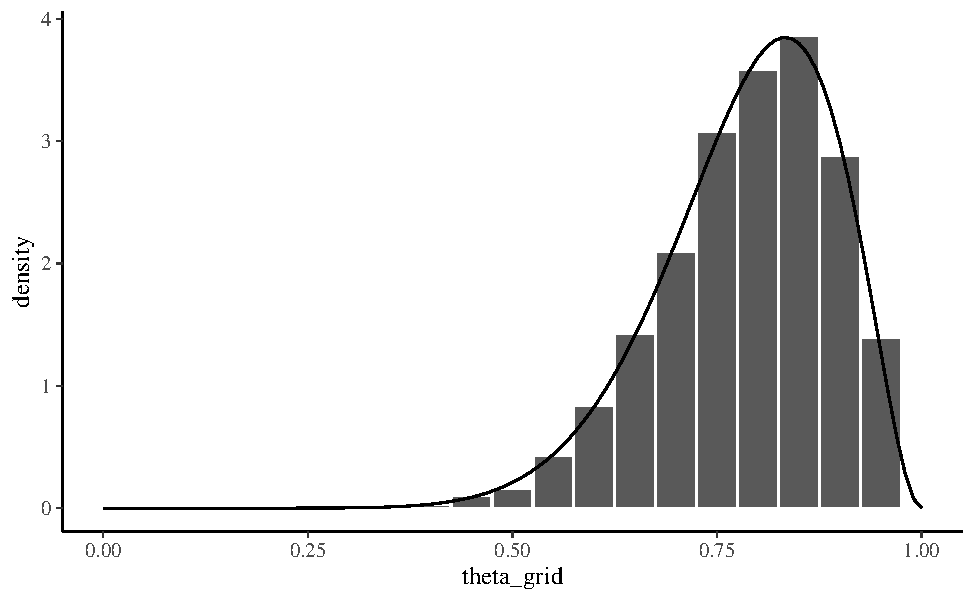
\includegraphics{ds4psy_files/figure-latex/grid-method-100points-posterior-plot-and-correct-posterior-1} 

}

\caption{Campionamento dalla  distribuzione a posteriori discretizzata ottenuta con il metodo grid-based per $y$ = 9 successi in 10 prove Bernoulliane, con distribuzione a priori $\mbox{Beta}(2, 2)$. È stata utilizzata una griglia di $n$ = 100 punti. All'istogramma è stata sovrapposta la corretta distribuzione a posteriori, ovvero la densità $\mbox{Beta}(11, 3)$.}\label{fig:grid-method-100points-posterior-plot-and-correct-posterior}
\end{figure}

In conclusione, il metodo basato su griglia è molto intuitivo e non richiede particolari competenze di programmazione per essere implementato. Inoltre, fornisce un risultato che, per tutti gli scopi pratici, può essere considerato come un campione casuale estratto da \(p(\theta \mid y)\). Tuttavia, anche se tale metodo fornisce risultati accuratissimi, esso ha un uso limitato. A causa della \emph{maledizione della dimensionalità}\footnote{Per capire cosa sia la maledizione della dimensionalità, supponiamo di utilizzare una griglia di 100 punti equispaziati. Nel caso di un solo parametro, è necessario calcolare 100 valori. Per due parametri devono essere calcolari \(100^2\) valori. Ma già per 10 parametri è necessario calcolare \(10^{10}\) valori -- è facile capire che una tale quantità di calcoli è troppo grande anche per un computer molto potente. Per modelli che richiedono la stima di un numero non piccolo di parametri è dunque necessario procedere in un altro modo.}, tale metodo può solo essere solo nel caso di semplici modelli statistici, con non più di due parametri. Nella pratica concreta tale metodo viene dunque sostituito da altre tecniche più efficienti in quanto, anche nei più comuni modelli utilizzati in psicologia, vengono solitamente stimati centinaia se non migliaia di parametri.

\hypertarget{approssimazione-quadratica}{%
\section{Approssimazione quadratica}\label{approssimazione-quadratica}}

L'approssimazione quadratica è un metodo analitico approssimato che può essere usato per superare il problema della ``maledizione della dimensionalità''. La motivazione di tale metodo è la seguente. Sappiamo che, in generale, la regione della distribuzione a posteriori che si trova in prossimità del suo massimo può essere ben approssimata dalla forma di una distribuzione Normale.\footnote{Descrivere la distribuzione a posteriori mediante la distribuzione Normale significa utilizzare un'approssimazione che viene, appunto, chiamata ``quadratica'' (tale approssimazione si dice quadratica perché il logaritmo di una distribuzione gaussiana forma una parabola e la parabola è una funzione quadratica -- dunque, mediante questa approssimazione descriviamo il logaritmo della distribuzione a posteriori mediante una parabola).}

L'approssimazione quadratica si pone due obiettivi.

\begin{enumerate}
\def\labelenumi{\arabic{enumi}.}
\tightlist
\item
  Trovare la moda della distribuzione a posteriori. Ci sono varie procedure di ottimizzazione, implementate in \(\R\), in grado di trovare il massimo di una distribuzione.
\item
  Stimare la curvatura della distribuzione in prossimità della moda. Una stima della curvatura è sufficiente per trovare un'approssimazione quadratica dell'intera distribuzione. In alcuni casi, questi calcoli possono essere fatti seguendo una procedura analitica, ma solitamente vengono usate delle tecniche numeriche.
\end{enumerate}

Una descrizione della distribuzione a posteriori ottenuta mediante l'approssimazione quadratica si ottiene mediante la funzione \texttt{quap()} contenuta nel pacchetto \texttt{rethinking}:\footnote{Il pacchetto \texttt{rethinking} è stato creato da \citet{McElreath_rethinking} per accompagnare il suo testo \emph{Statistical Rethinking}\(^2\). Per l'installazione si veda \url{https://github.com/rmcelreath/rethinking}.}

\begin{Shaded}
\begin{Highlighting}[]
\FunctionTok{suppressPackageStartupMessages}\NormalTok{(}\FunctionTok{library}\NormalTok{(}\StringTok{"rethinking"}\NormalTok{))}

\NormalTok{mod }\OtherTok{\textless{}{-}} \FunctionTok{quap}\NormalTok{(}
  \FunctionTok{alist}\NormalTok{(}
\NormalTok{  N }\SpecialCharTok{\textasciitilde{}} \FunctionTok{dbinom}\NormalTok{(N }\SpecialCharTok{+}\NormalTok{ P, p), }\CommentTok{\# verosimiglianza binomiale}
\NormalTok{  p }\SpecialCharTok{\textasciitilde{}} \FunctionTok{dbeta}\NormalTok{(}\DecValTok{2}\NormalTok{, }\DecValTok{10}\NormalTok{) }\CommentTok{\# distribuzione a priori Beta(2, 10)}
\NormalTok{  ),}
  \AttributeTok{data =} \FunctionTok{list}\NormalTok{(}\AttributeTok{N =} \DecValTok{23}\NormalTok{, }\AttributeTok{P =} \DecValTok{7}\NormalTok{)}
\NormalTok{)}
\end{Highlighting}
\end{Shaded}

Un sommario dell'approssimazione quadratica è fornito da

\begin{Shaded}
\begin{Highlighting}[]
\FunctionTok{precis}\NormalTok{(mod, }\AttributeTok{prob =} \FloatTok{0.95}\NormalTok{)}
\CommentTok{\#\textgreater{}   mean      sd   2.5\%  97.5\%}
\CommentTok{\#\textgreater{} p  0.6 0.07746 0.4482 0.7518}
\end{Highlighting}
\end{Shaded}

Qui sotto è fornito un confronto tra la corretta distribuzione a posteriori (linea continua) e l'approssimazione quadratica (linea trateggiata).

\begin{Shaded}
\begin{Highlighting}[]
\NormalTok{N }\OtherTok{\textless{}{-}} \DecValTok{23}
\NormalTok{P }\OtherTok{\textless{}{-}} \DecValTok{7}
\NormalTok{a }\OtherTok{\textless{}{-}}\NormalTok{ N }\SpecialCharTok{+} \DecValTok{2}
\NormalTok{b }\OtherTok{\textless{}{-}}\NormalTok{ P }\SpecialCharTok{+} \DecValTok{10}
\FunctionTok{curve}\NormalTok{(}\FunctionTok{dbeta}\NormalTok{(x, a, b), }\AttributeTok{from=}\DecValTok{0}\NormalTok{, }\AttributeTok{to=}\DecValTok{1}\NormalTok{, }\AttributeTok{ylab=}\StringTok{"Densità"}\NormalTok{)}
\CommentTok{\# approssimazione quadratica}
\FunctionTok{curve}\NormalTok{(}
  \FunctionTok{dnorm}\NormalTok{(x, a}\SpecialCharTok{/}\NormalTok{(a}\SpecialCharTok{+}\NormalTok{b), }\FunctionTok{sqrt}\NormalTok{((a}\SpecialCharTok{*}\NormalTok{b)}\SpecialCharTok{/}\NormalTok{((a}\SpecialCharTok{+}\NormalTok{b)}\SpecialCharTok{\^{}}\DecValTok{2}\SpecialCharTok{*}\NormalTok{(a}\SpecialCharTok{+}\NormalTok{b}\SpecialCharTok{+}\DecValTok{1}\NormalTok{)))),}
  \AttributeTok{lty =} \DecValTok{2}\NormalTok{,}
  \AttributeTok{add =} \ConstantTok{TRUE}
\NormalTok{)}
\end{Highlighting}
\end{Shaded}

\begin{center}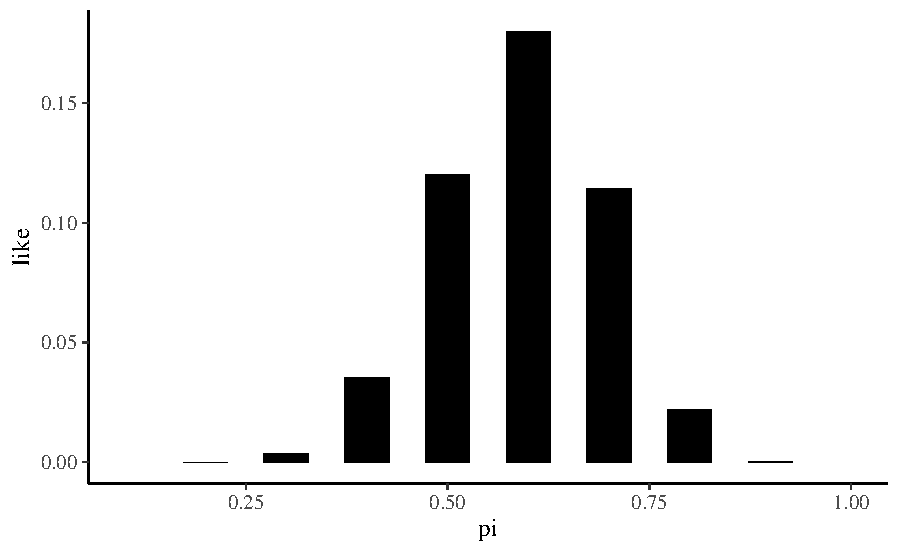
\includegraphics{ds4psy_files/figure-latex/unnamed-chunk-15-1} \end{center}

Il grafico precedente mostra che l'approssimazione quadratica fornisce risultati soddisfacenti. Tali risultati sono simili (o identici) a quelli ottenuti con il metodo \emph{grid-based}, con il vantaggio aggiuntivo di disporre di una serie di funzioni \(\R\) in grado di svolgere i calcoli per noi. In realtà, però, l'approssimazione quadratica è poco usata perché, per problemi complessi, è più conveniente fare ricorso ai metodi Monte Carlo basati su Catena di Markov (MCMC) che verranno descritti nel Paragrafo successivo.

\hypertarget{chapter-simulazioneMC}{%
\section{Metodo Monte Carlo}\label{chapter-simulazioneMC}}

I metodi più ampiamente adottati nell'analisi bayesiana per la costruzione della distribuzione a posteriori per modelli complessi sono i metodi di campionamento Monte Carlo basati su catena di Markov (\emph{Markov Chain Monte Carlo}, MCMC). Tali metodi consentono al ricercatore di decidere quali distribuzioni a priori e quali distribuzioni di verosimiglianza usare sulla base di considerazioni teoriche soltanto, senza dovere preoccuparsi di altri vincoli. Dato che è basata su metodi computazionalmente intensivi, la stima numerica MCMC della funzione a posteriori può essere svolta soltanto mediante software. In anni recenti i metodi Bayesiani di analisi dei dati sono diventati sempre più popolari proprio perché la potenza di calcolo necessaria per svolgere tali calcoli è ora alla portata di tutti. Questo non era vero solo pochi decenni fa.

\hypertarget{integration-mc}{%
\subsection{Integrazione di Monte Carlo}\label{integration-mc}}

Il termine Monte Carlo si riferisce al fatto che la computazione fa ricorso ad un ripetuto campionamento casuale attraverso la generazione di sequenze di numeri casuali. Una delle sue applicazioni più potenti è il calcolo degli integrali mediante simulazione numerica. Data una successione di realizzazioni indipendenti \(y^{(1)}, y^{(2)},\dots, y^{(T)}\) da una distribuzione \(p(y)\) con media \(\mu\) abbiamo che

\[
\E(Y) = \int y p(y) dy \approx \frac{1}{T} \sum_{i=1}^T y^{(t)}.
\] In altre parole, l'aspettazione teorica di \(Y\) può essere approssimata dalla media campionaria di un insieme di realizzazioni indipendenti ricavate da \(p(y)\). Per la Legge Forte dei Grandi Numeri, l'approssimazione diventa arbitrariamente esatta per \(T \rightarrow \infty\). L'integrazione Monte Carlo può essere utilizzata anche per la valutazione di integrali più complessi.

Quello che è stato detto sopra non è altro che un modo sofisticato per dire che, se vogliamo calcolare un'approssimazione del valore atteso di una variabile casuale, non dobbiamo fare altro che la media aritmetica di un grande numero di realizzazioni della variabile casuale. Come è facile intuire, l'approssimazione migliora al crescere del numero di dati che abbiamo a disposizione.

Un'altra importante funzione di \(Y\) è la funzione indicatore, \(I(l < Y < u)\), che assume valore 1 se \(Y\) giace nell'intervallo \((l,u)\) e 0 altrimenti. Il valore di aspettazione di \(I(l < X < u)\) rispetto a \(p(x)\) dà la probabilità che \(Y\) rientri nell'intervallo specificato, \(Pr(l < T < u)\), e può essere approssimato usando l'integrazione Monte Carlo, ovvero prendendo la media campionaria del valore della funzione indicatore per ogni realizzazione \(y^{(t)}\). È semplice vedere come

\[
Pr(l < Y < u) \approx \frac{\text{numero di realizzazioni } y^{(t)} \in (l, u)}{T}.
\]

L'integrazione di Monte Carlo può essere usata per approssimare la distribuzione a posteriori richiesta da un'analisi Bayesiana: una stima di \(p(\theta \mid y)\) viene ottenuta mediante un grande numero di campioni casuali dalla distribuzionea a posteriori.

\hypertarget{un-esempio-concreto}{%
\subsection{Un esempio concreto}\label{un-esempio-concreto}}

Per introdurre i metodi MCMC consideriamo il caso di una verosimiglianza Binomiale e di una distribuzione a priori Beta. Sappiamo che, in tali circostanze, viene prodotta una distribuzione a posteriori Beta (si veda il capitolo \ref{chapter-distr-coniugate}). Con una simulazione \(\R\) è dunque facile ricavare dei campioni causali dalla distribuzione a posteriori. Maggiore è il numero di campioni, migliore sarà l'approssimazione della distribuzione a posteriori.

Consideriamo nuovamente i dati di \citet{zetschefuture2019} (23 ``successi'' in 30 prove Bernoulliane) e applichiamo a quei dati lo stesso modello del Capitolo \ref{chapter-distr-coniugate}:

\begin{align}
y \mid \theta, n &\sim \Bin(y = 23, n = 30 \mid \theta) \notag\\
\theta_{prior} &\sim \mbox{Beta}(2, 10) \notag\\
\theta_{post}  &\sim \mbox{Beta}(y + a = 23 + 2 = 25, n - y + b = 30 - 23 + 10 = 17), \notag
\end{align}

Poniamoci il problema di stimare il valore della media a posteriori di \(\theta\). Nel caso presente, il risultato esatto è

\[
\bar{\theta}_{post} = \frac{\alpha}{\alpha + \beta} = \frac{25}{25 + 17} \approx 0.5952.
\] Dato che la distribuzione a posteriori di \(\theta\) è \(\mbox{Beta}(25, 17)\), possiamo estrarre un campione casuale di osservazioni da tale distribuzione e calcolare la media:

\begin{Shaded}
\begin{Highlighting}[]
\FunctionTok{set.seed}\NormalTok{(}\DecValTok{7543897}\NormalTok{)}
\FunctionTok{print}\NormalTok{(}\FunctionTok{mean}\NormalTok{(}\FunctionTok{rbeta}\NormalTok{(}\FloatTok{1e2}\NormalTok{, }\AttributeTok{shape1 =} \DecValTok{25}\NormalTok{, }\AttributeTok{shape2 =} \DecValTok{17}\NormalTok{)), }\DecValTok{6}\NormalTok{)}
\CommentTok{\#\textgreater{} [1] 0.587548}
\end{Highlighting}
\end{Shaded}

È ovvio che l'approssimazione migliora all'aumentare del numero di osservazioni estratte dalla distribuzione a posteriori (legge dei grandi numeri):

\begin{Shaded}
\begin{Highlighting}[]
\FunctionTok{print}\NormalTok{(}\FunctionTok{mean}\NormalTok{(}\FunctionTok{rbeta}\NormalTok{(}\FloatTok{1e3}\NormalTok{, }\AttributeTok{shape1 =} \DecValTok{25}\NormalTok{, }\AttributeTok{shape2 =} \DecValTok{17}\NormalTok{)), }\DecValTok{6}\NormalTok{)}
\CommentTok{\#\textgreater{} [1] 0.597659}
\end{Highlighting}
\end{Shaded}

\begin{Shaded}
\begin{Highlighting}[]
\FunctionTok{print}\NormalTok{(}\FunctionTok{mean}\NormalTok{(}\FunctionTok{rbeta}\NormalTok{(}\FloatTok{1e4}\NormalTok{, }\AttributeTok{shape1 =} \DecValTok{25}\NormalTok{, }\AttributeTok{shape2 =} \DecValTok{17}\NormalTok{)), }\DecValTok{6}\NormalTok{)}
\CommentTok{\#\textgreater{} [1] 0.595723}
\end{Highlighting}
\end{Shaded}

\begin{Shaded}
\begin{Highlighting}[]
\FunctionTok{print}\NormalTok{(}\FunctionTok{mean}\NormalTok{(}\FunctionTok{rbeta}\NormalTok{(}\FloatTok{1e5}\NormalTok{, }\AttributeTok{shape1 =} \DecValTok{25}\NormalTok{, }\AttributeTok{shape2 =} \DecValTok{17}\NormalTok{)), }\DecValTok{6}\NormalTok{)}
\CommentTok{\#\textgreater{} [1] 0.595271}
\end{Highlighting}
\end{Shaded}

Quando il numero di osservazioni (possiamo anche chiamarle ``campioni'') tratte dalla distribuzione a posteriori è molto grande, la distribuzione di tali campioni converge alla densità della popolazione (si veda l'Appendice \ref{integration-mc}).\footnote{Si noti, naturalmente, che il numero dei campioni di simulazione è controllato dal ricercatore; è totalmente diverso dalla dimensione del campione che è fissa ed è una proprietà dei dati.}

Inoltre, le statistiche descrittive (es. media, moda, varianza, eccetera) dei campioni estratti dalla distribuzione a posteriori convergeranno ai corrispondenti valori della distribuzione a posteriori. La figura \ref{fig:mcmc-chains-1} mostra come, all'aumentare del numero di repliche, la media, la mediana, la deviazione standard e l'asimmetria convergono ai veri valori della distribuzione a posteriori (linee rosse tratteggiate).

\begin{figure}[h]

{\centering 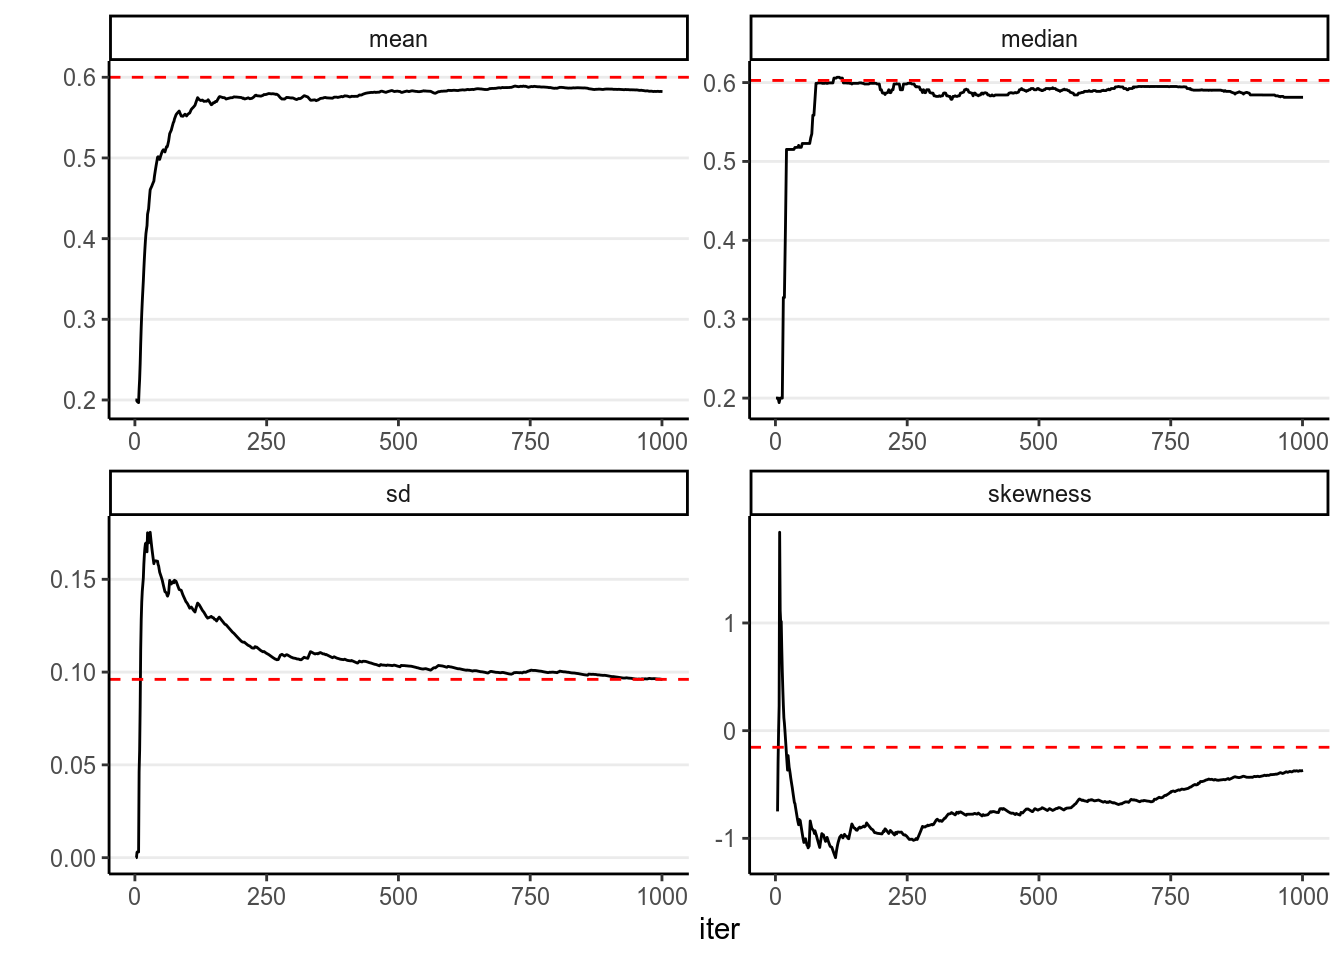
\includegraphics[width=0.8\linewidth]{/Users/corrado/_repositories/ds4psy/images/mcmc-chains-1} 

}

\caption{Convergenza delle simulazioni Monte Carlo.}\label{fig:mcmc-chains-1}
\end{figure}

\hypertarget{metodi-mc-basati-su-catena-di-markov}{%
\subsection{Metodi MC basati su Catena di Markov}\label{metodi-mc-basati-su-catena-di-markov}}

Nel Paragrafo \ref{chapter-simulazioneMC} la simulazione Monte Carlo funzionava perché

\begin{itemize}
\tightlist
\item
  sapevamo che la distribuzione a posteriori era una \(\mbox{Beta}(25, 17)\),
\item
  era possibile usare le funzioni \(\R\) per estrarre campioni casuali da tale distribuzione.
\end{itemize}

Tuttavia, capita raramente di usare una distribuzione a priori coniugata alla verosimiglianza, quindi in generale le due condizioni descritte sopra non si applicano. Ad esempio, nel caso di una verosimiglianza binomiale e una distribuzione a priori Normale, la distribuzione a posteriori di \(\theta\) è

\[
p(\theta \mid y) = \frac{\mathrm{e}^{-(\theta - 1 / 2)^2} \theta^y (1 - \theta)^{n - y}} {\int_0^1 \mathrm{e}^{-(t - 1 / 2)^2} t^y (1 - t)^{n - y} dt}.
\]

Una tale distribuzione non è implementata in \(\R\) e dunque non possiamo campionare da \(p(\theta \mid y)\). Per fortuna, gli algoritmi MCMC consentono il campionamento da una distribuzione a posteriori \emph{senza che sia necessario conoscere la rappresentazione analitica di una tale distribuzione}. I metodi Monte Carlo basati su catena di Markov consentono di costruire sequenze di punti (detti catene di Markov) nello spazio dei parametri le cui densità sono proporzionali alla distribuzione a posteriori --- in altre parole, dopo aver simulato un grande numero di passi della catena si possono usare i valori così generati come se fossero un campione casuale della distribuzione a posteriori. Le tecniche MCMC sono attualmente il metodo computazionale maggiormente utilizzato per risolvere i problemi di inferenza bayesiana. Un'introduzione alle catene di Markov è fornita nell'Appendice \ref{markov-chains}.

\hypertarget{campionamento-mediante-algoritmi-mcmc}{%
\subsection{Campionamento mediante algoritmi MCMC}\label{campionamento-mediante-algoritmi-mcmc}}

Un modo generale per ottenere una catena di Markov la cui distribuzione equivale alla distribuzione a posteriori \(p(\theta \mid y)\) è quello di usare l'algoritmo di Metropolis. L'algoritmo di Metropolis è il primo algoritmo MCMC che è stato proposto, ed è applicabile ad una grande varietà di problemi inferenziali di tipo bayesiano. Tale algoritmo è stato in seguito sviluppato allo scopo di renderlo via via più efficiente. Lo presentiamo qui in una forma intuitiva.

\hypertarget{una-passeggiata-casuale-sui-numeri-naturali}{%
\subsection{Una passeggiata casuale sui numeri naturali}\label{una-passeggiata-casuale-sui-numeri-naturali}}

Per introdurre l'algoritmo di di Metropolis considereremo il campionamento da una distribuzione discreta.\footnote{Seguiamo qui la trattazione di \citet{albert2019probability}. Per una presentazione intuitiva dell'algoritmo di Metropolis, si vedano anche \citet{doing_bayesian_data_an}; \citet{McElreath_rethinking}.} Supponiamo di definire una distribuzione di probabilità discreta sugli interi \(1,\dots, K\). Scriviamo in \(\R\) la funzione \texttt{pd()} che assegna ai valori \(1,\dots, 8\) delle probabilità proporzionali a 5, 10, 4, 4, 20, 20, 12 e 5.

\begin{Shaded}
\begin{Highlighting}[]
\NormalTok{pd }\OtherTok{\textless{}{-}} \ControlFlowTok{function}\NormalTok{(x)\{}
\NormalTok{  values }\OtherTok{\textless{}{-}} \FunctionTok{c}\NormalTok{(}\DecValTok{5}\NormalTok{, }\DecValTok{10}\NormalTok{, }\DecValTok{4}\NormalTok{, }\DecValTok{4}\NormalTok{, }\DecValTok{20}\NormalTok{, }\DecValTok{20}\NormalTok{, }\DecValTok{12}\NormalTok{, }\DecValTok{5}\NormalTok{)}
  \FunctionTok{ifelse}\NormalTok{(}
\NormalTok{    x }\SpecialCharTok{\%in\%} \DecValTok{1}\SpecialCharTok{:}\FunctionTok{length}\NormalTok{(values),}
\NormalTok{    values[x] }\SpecialCharTok{/} \FunctionTok{sum}\NormalTok{(values),}
    \DecValTok{0}
\NormalTok{  )}
\NormalTok{\}}
\NormalTok{prob\_dist }\OtherTok{\textless{}{-}} \FunctionTok{tibble}\NormalTok{(}
  \AttributeTok{x =} \DecValTok{1}\SpecialCharTok{:}\DecValTok{8}\NormalTok{,}
  \AttributeTok{prob =} \FunctionTok{pd}\NormalTok{(}\DecValTok{1}\SpecialCharTok{:}\DecValTok{8}\NormalTok{)}
\NormalTok{)}
\end{Highlighting}
\end{Shaded}

La figura \ref{fig:formetropolisdistr} illustra la distribuzione di probabilità che è stata generata.

\begin{Shaded}
\begin{Highlighting}[]
\NormalTok{x }\OtherTok{\textless{}{-}} \DecValTok{1}\SpecialCharTok{:}\DecValTok{8}
\NormalTok{prob\_dist }\SpecialCharTok{\%\textgreater{}\%}
  \FunctionTok{ggplot}\NormalTok{(}\FunctionTok{aes}\NormalTok{(}\AttributeTok{x =}\NormalTok{ x, }\AttributeTok{y =}\NormalTok{ prob)) }\SpecialCharTok{+}
  \FunctionTok{geom\_bar}\NormalTok{(}\AttributeTok{stat =} \StringTok{"identity"}\NormalTok{, }\AttributeTok{width =} \FloatTok{0.06}\NormalTok{) }\SpecialCharTok{+}
  \FunctionTok{scale\_x\_continuous}\NormalTok{(}\StringTok{"x"}\NormalTok{, }\AttributeTok{labels =} \FunctionTok{as.character}\NormalTok{(x), }\AttributeTok{breaks =}\NormalTok{ x) }\SpecialCharTok{+}
  \FunctionTok{labs}\NormalTok{(}
    \AttributeTok{y =} \StringTok{"Probabilità"}\NormalTok{,}
    \AttributeTok{x =} \StringTok{"X"}
\NormalTok{  )}
\end{Highlighting}
\end{Shaded}

\begin{figure}[h]

{\centering 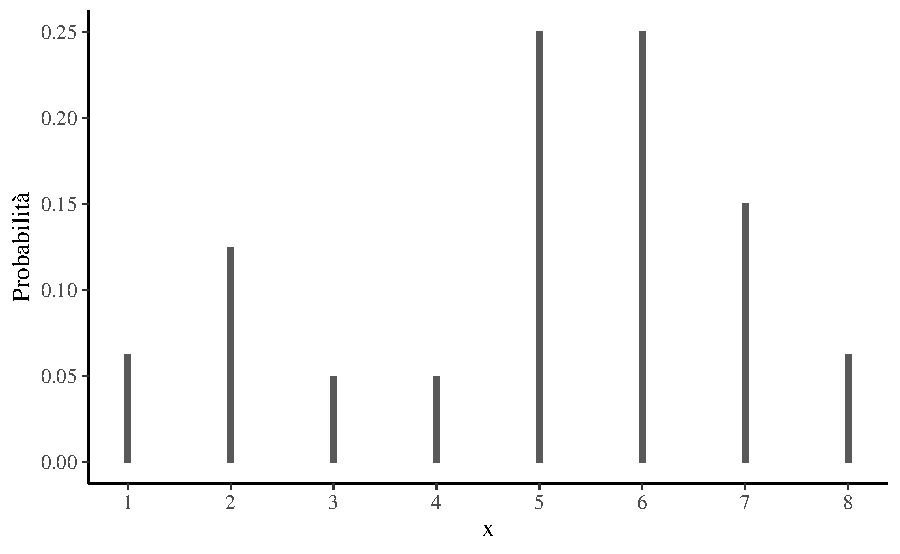
\includegraphics{ds4psy_files/figure-latex/formetropolisdistr-1} 

}

\caption{Distribuzione di massa di probabilità per una variabile casuale avente valori 1, 2, ..., 8.}\label{fig:formetropolisdistr}
\end{figure}

L'algoritmo di Metropolis corrisponde alla seguente passeggiata casuale.

\begin{enumerate}
\def\labelenumi{\arabic{enumi}.}
\tightlist
\item
  L'algoritmo inizia con un valore iniziale qualsiasi da 1 a \(K=8\) della variabile casuale.
\item
  Per simulare il valore successivo della sequenza, lanciamo una moneta equilibrata. Se esce testa, consideriamo come valore candidato il valore immediatamente precedente al valore corrente nella sequenza \(1, \dots, 8\); se esce croce, il valore candidato sarà il valore immediatamente successivo al valore corrente nella sequenza.
\item
  Calcoliamo il rapporto tra la probabilità del valore candidato e la probabilità del valore corrente:
\end{enumerate}

\[
R = \frac{pd(\text{valore candidato})}{pd(\text{valore corrente})}.
\]

\begin{enumerate}
\def\labelenumi{\arabic{enumi}.}
\setcounter{enumi}{3}
\tightlist
\item
  Estraiamo un numero a caso \(\in [0, 1]\). Se tale valore è minore di \(R\) accettiamo il valore candidato come valore successivo della catena markoviana; altrimenti il valore successivo della catena rimane il valore corrente.
\end{enumerate}

I passi da 1 a 4 definiscono una catena di Markov irriducibile e aperiodica sui valori di stato \(\{1, 2,\dots, 8\}\), dove il passo 1 fornisce il valore iniziale della catena e i passi da 2 a 4 definiscono la matrice di transizione \(P\). Un modo di campionare da una distribuzione di massa di probabilità \texttt{pd} consiste nell'iniziare da una posizione qualsiasi e eseguire una passeggiata casuale costituita da un grande numero di passi, ripetendo le fasi 2, 3 e 4 dell'algoritmo di Metropolis. Dopo un grande numero di passi, la distribuzione dei valori della catena markoviana approssimerà la distribuzione di probabilità \texttt{pd}.

La funzione \texttt{random\_walk()} implementa l'algoritmo di Metropolis. Tale funzione richiede in input la distribuzione di probabilità \texttt{pd}, la posizione di partenza \texttt{start} e il numero di passi dell'algoritmo \texttt{num\_steps}.

\begin{Shaded}
\begin{Highlighting}[]
\NormalTok{random\_walk }\OtherTok{\textless{}{-}} \ControlFlowTok{function}\NormalTok{(pd, start, num\_steps)\{}
\NormalTok{  y }\OtherTok{\textless{}{-}} \FunctionTok{rep}\NormalTok{(}\DecValTok{0}\NormalTok{, num\_steps)}
\NormalTok{  current }\OtherTok{\textless{}{-}}\NormalTok{ start}
  \ControlFlowTok{for}\NormalTok{ (j }\ControlFlowTok{in} \DecValTok{1}\SpecialCharTok{:}\NormalTok{num\_steps)\{}
\NormalTok{    candidate }\OtherTok{\textless{}{-}}\NormalTok{ current }\SpecialCharTok{+} \FunctionTok{sample}\NormalTok{(}\FunctionTok{c}\NormalTok{(}\SpecialCharTok{{-}}\DecValTok{1}\NormalTok{, }\DecValTok{1}\NormalTok{), }\DecValTok{1}\NormalTok{)}
\NormalTok{    prob }\OtherTok{\textless{}{-}} \FunctionTok{pd}\NormalTok{(candidate) }\SpecialCharTok{/} \FunctionTok{pd}\NormalTok{(current)}
    \ControlFlowTok{if}\NormalTok{ (}\FunctionTok{runif}\NormalTok{(}\DecValTok{1}\NormalTok{) }\SpecialCharTok{\textless{}}\NormalTok{ prob)}
\NormalTok{      current }\OtherTok{\textless{}{-}}\NormalTok{ candidate}
\NormalTok{    y[j] }\OtherTok{\textless{}{-}}\NormalTok{ current}
\NormalTok{  \}}
  \FunctionTok{return}\NormalTok{(y)}
\NormalTok{\}}
\end{Highlighting}
\end{Shaded}

Di seguito, implementiamo l'algoritmo di Metropolis utilizzando, quale valore iniziale, \(X=4\). Ripetiamo la simulazione 10,000 volte.

\begin{Shaded}
\begin{Highlighting}[]
\NormalTok{out }\OtherTok{\textless{}{-}} \FunctionTok{random\_walk}\NormalTok{(pd, }\DecValTok{4}\NormalTok{, }\FloatTok{1e4}\NormalTok{)}

\NormalTok{S }\OtherTok{\textless{}{-}} \FunctionTok{tibble}\NormalTok{(out) }\SpecialCharTok{\%\textgreater{}\%}
  \FunctionTok{group\_by}\NormalTok{(out) }\SpecialCharTok{\%\textgreater{}\%}
  \FunctionTok{summarize}\NormalTok{(}
    \AttributeTok{N =} \FunctionTok{n}\NormalTok{(),}
    \AttributeTok{Prob =}\NormalTok{ N }\SpecialCharTok{/} \DecValTok{10000}
\NormalTok{  )}

\NormalTok{prob\_dist2 }\OtherTok{\textless{}{-}} \FunctionTok{rbind}\NormalTok{(}
\NormalTok{  prob\_dist,}
  \FunctionTok{tibble}\NormalTok{(}
    \AttributeTok{x =}\NormalTok{ S}\SpecialCharTok{$}\NormalTok{out,}
    \AttributeTok{prob =}\NormalTok{ S}\SpecialCharTok{$}\NormalTok{Prob}
\NormalTok{  )}
\NormalTok{)}
\NormalTok{prob\_dist2}\SpecialCharTok{$}\NormalTok{Type }\OtherTok{\textless{}{-}} \FunctionTok{rep}\NormalTok{(}
  \FunctionTok{c}\NormalTok{(}\StringTok{"Prob. corrette"}\NormalTok{, }\StringTok{"Prob. simulate"}\NormalTok{),}
  \AttributeTok{each =} \DecValTok{8}
\NormalTok{)}
\end{Highlighting}
\end{Shaded}

\begin{Shaded}
\begin{Highlighting}[]
\NormalTok{x }\OtherTok{\textless{}{-}} \DecValTok{1}\SpecialCharTok{:}\DecValTok{8}
\NormalTok{prob\_dist2 }\SpecialCharTok{\%\textgreater{}\%}
  \FunctionTok{ggplot}\NormalTok{(}\FunctionTok{aes}\NormalTok{(}\AttributeTok{x =}\NormalTok{ x, }\AttributeTok{y =}\NormalTok{ prob, }\AttributeTok{fill =}\NormalTok{ Type)) }\SpecialCharTok{+}
  \FunctionTok{geom\_bar}\NormalTok{(}
    \AttributeTok{stat =} \StringTok{"identity"}\NormalTok{,}
    \AttributeTok{width =} \FloatTok{0.1}\NormalTok{,}
    \AttributeTok{position =} \FunctionTok{position\_dodge}\NormalTok{(}\FloatTok{0.3}\NormalTok{)}
\NormalTok{  ) }\SpecialCharTok{+}
  \FunctionTok{scale\_x\_continuous}\NormalTok{(}
    \StringTok{"x"}\NormalTok{,}
    \AttributeTok{labels =} \FunctionTok{as.character}\NormalTok{(x),}
    \AttributeTok{breaks =}\NormalTok{ x}
\NormalTok{  ) }\SpecialCharTok{+}
  \FunctionTok{scale\_fill\_manual}\NormalTok{(}\AttributeTok{values =} \FunctionTok{c}\NormalTok{(}\StringTok{"black"}\NormalTok{, }\StringTok{"gray80"}\NormalTok{)) }\SpecialCharTok{+}
  \FunctionTok{theme}\NormalTok{(}\AttributeTok{legend.title =} \FunctionTok{element\_blank}\NormalTok{()) }\SpecialCharTok{+}
  \FunctionTok{labs}\NormalTok{(}
    \AttributeTok{y =} \StringTok{"Probabilità"}\NormalTok{,}
    \AttributeTok{x =} \StringTok{"X"}
\NormalTok{  )}
\end{Highlighting}
\end{Shaded}

\begin{figure}[h]

{\centering 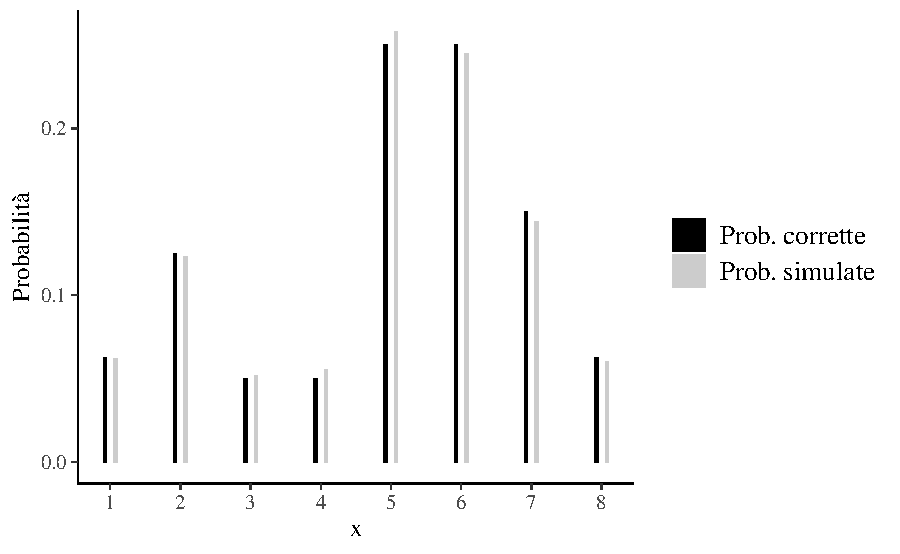
\includegraphics{ds4psy_files/figure-latex/metropolishistogramsim-1} 

}

\caption{L'istogramma confronta i valori prodotti dall'algoritmo di Metropolis con i corretti valori della distribuzione di massa di probabilità.}\label{fig:metropolishistogramsim}
\end{figure}

La figura \ref{fig:metropolishistogramsim} confronta l'istogramma dei valori simulati dalla passeggiata casuale con l'effettiva distribuzione di probabilità \texttt{pd}. Si noti la somiglianza tra le due distribuzioni.

\hypertarget{lalgoritmo-di-metropolis}{%
\subsection{L'algoritmo di Metropolis}\label{lalgoritmo-di-metropolis}}

Vediamo ora come l'algoritmo di Metropolis possa venire usato per generare una catena di Markov irriducibile e aperiodica per la quale la distribuzione stazionaria è uguale alla distribuzione a posteriori di interesse.\footnote{Una illustrazione visiva di come si svolge il processo di ``esplorazione'' dell'algoritmo di Metropolis è fornita in questo \href{https://elevanth.org/blog/2017/11/28/build-a-better-markov-chain/}{post}.} In termini generali, l'algoritmo di Metropolis include due fasi.

\begin{itemize}
\tightlist
\item
  \emph{Fase 1.} La selezione di un valore candidato \(\theta'\) del parametro mediante il campionamento da una distribuzione proposta.
\item
  \emph{Fase 2.} La decisione tra la possibilità di accettare il valore candidato \(\theta^{(m+1)} = \theta'\) o di mantenere il valore corrente \(\theta^{(m+1)} = \theta\) sulla base del seguente criterio:

  \begin{itemize}
  \tightlist
  \item
    se \(\mathcal{L}(\theta' \mid y)p(\theta') > \mathcal{L}(\theta \mid y)p(\theta)\) il valore candidato viene sempre accettato;
  \item
    altrimenti il valore candidato viene accettato solo in una certa proporzione di casi.
  \end{itemize}
\end{itemize}

Esaminiamo ora nei dettagli il funzionamento dell'algoritmo di Metropolis.

\begin{enumerate}
\def\labelenumi{(\alph{enumi})}
\item
  Si inizia con un punto arbitrario \(\theta^{(1)}\), quindi il primo valore della catena di Markov \(\theta^{(1)}\) può corrispondere semplicemente ad un valore a caso tra i valori possibili del parametro.
\item
  Per ogni passo successivo della catena, \(m + 1\), si campiona un valore candidato \(\theta'\) da una distribuzione proposta: \(\theta' \sim \Pi(\theta)\). La distribuzione proposta può essere qualunque distribuzione, anche se, idealmente, è meglio che sia simile alla distribuzione a posteriori. In pratica, però, la distribuzione a posteriori è sconosciuta e quindi il valore \(\theta'\) viene campionato da una qualche distribuzione simmetrica centrata sul valore corrente \(\theta^{(m)}\) del parametro. Nell'esempio qui discusso, useremo la distribuzione gaussiana. Tale distribuzione sarà centrata sul valore corrente della catena e avrà una appropriata deviazione standard: \(\theta' \sim \mathcal{N}(\theta^{(m)}, \sigma)\). In pratica, questo significa che, se \(\sigma\) è piccola, il valore candidato \(\theta'\) sarà simile al valore corrente \(\theta^{(m)}\).
\item
  Una volta generato il valore candidato \(\theta'\) si calcola il rapporto tra la densità della distribuzione a posteriori non normalizzata nel punto \(\theta'\) {[}ovvero, il prodotto tra la verosimiglianza \(\mathcal{L}(y \mid \theta')\) nel punto \(\theta'\) e la distribuzione a priori nel punto \(\theta'\){]} e la densità della distribuzione a posteriori non normalizzata nel punto \(\theta^{(m)}\) {[}ovvero, il prodotto tra la verosimiglianza \(\mathcal{L}(y \mid \theta^{(m)})\) nel punto \(\theta^{(m)}\) e la distribuzione a priori nel punto \(\theta^{(m)}\){]}:
\end{enumerate}

\begin{equation}
\alpha = \frac{p(y \mid \theta') p(\theta')}{p(y \mid \theta^{(m)}) p(\theta^{(m)})}.
\label{eq:ratio-metropolis}
\end{equation}

Si noti che, essendo un rapporto, la \eqref{eq:ratio-metropolis} cancella la costante di normalizzazione.

\begin{enumerate}
\def\labelenumi{(\alph{enumi})}
\setcounter{enumi}{3}
\item
  Il rapporto \(\alpha\) viene utilizzato per decidere se accettare il valore candidato \(\theta'\), oppure se campionare un diverso candidato. Possiamo pensare al rapporto \(\alpha\) come alla risposta alla seguente domanda: alla luce dei dati, è più plausibile il valore candidato del parametro o il valore corrente? Se \(\alpha\) è maggiore di 1 ciò significa che il valore candidato è più plausibile del valore corrente; in tali circostanze il valore candidato viene sempre accettato. Altrimenti, si decide di accettare il valore candidato con una probabilità minore di 1, ovvero non sempre, ma soltanto con una probabilità uguale ad \(\alpha\). Se \(\alpha\) è uguale a 0.10, ad esempio, questo significa che la plausibilità a posteriori del valore candidato è 10 volte più piccola della plausibilità a posteriori del valore corrente. Dunque, il valore candidato verrà accettato solo nel 10\% dei casi. Come conseguenza di questa strategia di scelta, l'algoritmo di Metropolis ottiene un campione casuale dalla distribuzione a posteriori, dato che la probabilità di accettare il valore candidato è proporzionale alla densità del candidato nella distribuzione a posteriori. Dal punto di vista algoritmico, la procedura descritta sopra viene implementata confrontando il rapporto \(\alpha\) con un valore casuale estratto da una distribuzione uniforme \(\mbox{Unif}(0, 1)\). Se \(\alpha > u \sim \mbox{Unif}(0, 1)\) allora il punto candidato \(\theta'\) viene accettato e la catena si muove in quella nuova posizione, ovvero \(\theta^{(m+1)} = \theta'^{(m+1)}\). Altrimenti \(\theta^{(m+1)} = \theta^{(m)}\) e si campiona un nuovo valore candidato \(\theta'\).
\item
  Il passaggio finale dell'algoritmo calcola l'\emph{accettanza} in una specifica esecuzione dell'algoritmo, ovvero la proporzione dei valori candidati \(\theta'\) che sono stati accettati come valori successivi nella sequenza.
\end{enumerate}

L'algoritmo di Metropolis prende come input il numero \(M\) di passi da simulare, la deviazione standard \(\sigma\) della distribuzione proposta e la densità a priori, e ritorna come output la sequenza \(\theta^{(1)}, \theta^{(2)}, \dots, \theta^{(M)}\). La chiave del successo dell'algoritmo di Metropolis è il numero di passi fino a che la catena approssima la stazionarietà. Tipicamente i primi da 1000 a 5000 elementi sono scartati. Dopo un certo periodo \(k\) (detto di \emph{burn-in}), la catena di Markov converge ad una variabile casuale che è distribuita secondo la distribuzione a posteriori. In altre parole, i campioni del vettore \(\left(\theta^{(k+1)}, \theta^{(k+2)}, \dots, \theta^{(M)}\right)\) diventano campioni di \(p(\theta \mid y)\).

\hypertarget{un-esempio-concreto-seconda-versione}{%
\subsection{Un esempio concreto (seconda versione)}\label{un-esempio-concreto-seconda-versione}}

Per fare un esempio concreto, consideriamo nuovamente i 30 pazienti esaminati da \citet{zetschefuture2019}. Di essi, 23 hanno manifestato aspettative distorte negativamente sul loro stato d'animo futuro. Utilizzando l'algoritmo di Metropolis, ci poniamo il problema di ottenere la stima a posteriori di \(\theta\) (probabilità di manifestare un'aspettativa distorta negativamente), dati 23 ``successi'' in 30 prove, imponendo su \(\theta\) la stessa distribuzione a priori usata nel Capitolo \ref{chapter-distr-coniugate}, ovvero \(\mbox{Beta}(2, 10)\).

Per calcolare la funzione di verosimiglianza, avendo fissato i dati di \citet{zetschefuture2019}, definiamo la funzione \texttt{likelihood()}

\begin{Shaded}
\begin{Highlighting}[]
\NormalTok{likelihood }\OtherTok{\textless{}{-}} \ControlFlowTok{function}\NormalTok{(param, }\AttributeTok{x =} \DecValTok{23}\NormalTok{, }\AttributeTok{N =} \DecValTok{30}\NormalTok{) \{}
  \FunctionTok{dbinom}\NormalTok{(x, N, param)}
\NormalTok{\}}
\end{Highlighting}
\end{Shaded}

che ritorna l'ordinata della verosimiglianza binomiale per ciascun valore del vettore \texttt{param} in input.

La distribuzione a priori \(\mbox{Beta}(2, 10)\) è implementata nella funzione \texttt{prior()}:

\begin{Shaded}
\begin{Highlighting}[]
\NormalTok{prior }\OtherTok{\textless{}{-}} \ControlFlowTok{function}\NormalTok{(param, }\AttributeTok{alpha =} \DecValTok{2}\NormalTok{, }\AttributeTok{beta =} \DecValTok{10}\NormalTok{) \{}
  \FunctionTok{dbeta}\NormalTok{(param, alpha, beta) }
\NormalTok{\}}
\end{Highlighting}
\end{Shaded}

Il prodotto della densità a priori e della verosimiglianza è implementato nella funzione \texttt{posterior()}:

\begin{Shaded}
\begin{Highlighting}[]
\NormalTok{posterior }\OtherTok{\textless{}{-}} \ControlFlowTok{function}\NormalTok{(param) \{}
  \FunctionTok{likelihood}\NormalTok{(param) }\SpecialCharTok{*} \FunctionTok{prior}\NormalTok{(param)}
\NormalTok{\}}
\end{Highlighting}
\end{Shaded}

L'Appendice \ref{es-pratico-zetsche-funzioni} mostra come un'approssimazione della distribuzione a posteriori \(p(\theta \mid y)\) per questi dati possa essere ottenuta mediante il metodo basato su griglia.

\hypertarget{implementazione}{%
\subsection{Implementazione}\label{implementazione}}

Per implementare l'algoritmo di Metropolis utilizzeremo una distribuzione proposta gaussiana. Il valore candidato sarà dunque un valore selezionato a caso da una gaussiana di parametri \(\mu\) uguale al valore corrente nella catena e \(\sigma = 0.9\). In questo esempio, la deviazione standard \(\sigma\) è stata scelta empiricamente in modo tale da ottenere una accettanza adeguata. L'accettanza ottimale è di circa 0.20 e 0.30 --- se l'accettanza è troppo grande, l'algoritmo esplora uno spazio troppo ristretto della distribuzione a posteriori.\footnote{L'accettanza dipende dalla distribuzione proposta: in generale, tanto più la distribuzione proposta è simile alla distribuzione target, tanto più alta diventa l'accettanza.}

\begin{Shaded}
\begin{Highlighting}[]
\NormalTok{proposal\_distribution }\OtherTok{\textless{}{-}} \ControlFlowTok{function}\NormalTok{(param) \{}
  \ControlFlowTok{while}\NormalTok{(}\DecValTok{1}\NormalTok{) \{}
\NormalTok{    res }\OtherTok{=} \FunctionTok{rnorm}\NormalTok{(}\DecValTok{1}\NormalTok{, }\AttributeTok{mean =}\NormalTok{ param, }\AttributeTok{sd =} \FloatTok{0.9}\NormalTok{)}
    \ControlFlowTok{if}\NormalTok{ (res }\SpecialCharTok{\textgreater{}} \DecValTok{0} \SpecialCharTok{\&}\NormalTok{ res }\SpecialCharTok{\textless{}} \DecValTok{1}\NormalTok{)}
      \ControlFlowTok{break}
\NormalTok{  \}}
\NormalTok{  res}
\NormalTok{\}}
\end{Highlighting}
\end{Shaded}

Nella presente implementazione del campionamento dalla distribuzione proposta è stato inserito un controllo che impone al valore candidato di essere incluso nell'intervallo {[}0, 1{]}.\footnote{Si possono trovare implementazioni dell'algoritmo di Metropolis più eleganti di quella presentata qui. Lo scopo dell'esercizio è quello di illustrare la logica soggiacente all'algoritmo di Metropolis, non quello di proporre un'implementazione efficente dell'algoritmo.}

L'algoritmo di Metropolis viene implementato nella seguente funzione:

\begin{Shaded}
\begin{Highlighting}[]
\NormalTok{run\_metropolis\_MCMC }\OtherTok{\textless{}{-}} \ControlFlowTok{function}\NormalTok{(startvalue, iterations) \{}
\NormalTok{  chain }\OtherTok{\textless{}{-}} \FunctionTok{vector}\NormalTok{(}\AttributeTok{length =}\NormalTok{ iterations }\SpecialCharTok{+} \DecValTok{1}\NormalTok{)}
\NormalTok{  chain[}\DecValTok{1}\NormalTok{] }\OtherTok{\textless{}{-}}\NormalTok{ startvalue}
  \ControlFlowTok{for}\NormalTok{ (i }\ControlFlowTok{in} \DecValTok{1}\SpecialCharTok{:}\NormalTok{iterations) \{}
\NormalTok{    proposal }\OtherTok{\textless{}{-}} \FunctionTok{proposal\_distribution}\NormalTok{(chain[i])}
\NormalTok{    r }\OtherTok{\textless{}{-}} \FunctionTok{posterior}\NormalTok{(proposal) }\SpecialCharTok{/} \FunctionTok{posterior}\NormalTok{(chain[i])}
    \ControlFlowTok{if}\NormalTok{ (}\FunctionTok{runif}\NormalTok{(}\DecValTok{1}\NormalTok{) }\SpecialCharTok{\textless{}}\NormalTok{ r) \{}
\NormalTok{      chain[i }\SpecialCharTok{+} \DecValTok{1}\NormalTok{] }\OtherTok{\textless{}{-}}\NormalTok{ proposal}
\NormalTok{    \} }\ControlFlowTok{else}\NormalTok{ \{}
\NormalTok{      chain[i }\SpecialCharTok{+} \DecValTok{1}\NormalTok{] }\OtherTok{\textless{}{-}}\NormalTok{ chain[i]}
\NormalTok{    \}}
\NormalTok{  \}}
\NormalTok{  chain}
\NormalTok{\}}
\end{Highlighting}
\end{Shaded}

Avendo definito le funzioni precedenti, generiamo una catena di valori \(\theta\):

\begin{Shaded}
\begin{Highlighting}[]
\FunctionTok{set.seed}\NormalTok{(}\DecValTok{123}\NormalTok{)}
\NormalTok{startvalue }\OtherTok{\textless{}{-}} \FunctionTok{runif}\NormalTok{(}\DecValTok{1}\NormalTok{, }\DecValTok{0}\NormalTok{, }\DecValTok{1}\NormalTok{)}
\NormalTok{niter }\OtherTok{\textless{}{-}} \FloatTok{1e4}
\NormalTok{chain }\OtherTok{\textless{}{-}} \FunctionTok{run\_metropolis\_MCMC}\NormalTok{(startvalue, niter)}
\end{Highlighting}
\end{Shaded}

Mediante le istruzioni precedenti otteniamo una catena di Markov costituita da 10,001 valori. Escludiamo i primi 5,000 valori considerati come burn-in. Ci restano dunque con 5,001 valori che verranno considerati come un campione casuale estratto dalla distribuzione a posteriori \(p(\theta \mid y)\).

L'accettanza è pari a

\begin{Shaded}
\begin{Highlighting}[]
\NormalTok{burnIn }\OtherTok{\textless{}{-}}\NormalTok{ niter }\SpecialCharTok{/} \DecValTok{2}
\NormalTok{acceptance }\OtherTok{\textless{}{-}} \DecValTok{1} \SpecialCharTok{{-}} \FunctionTok{mean}\NormalTok{(}\FunctionTok{duplicated}\NormalTok{(chain[}\SpecialCharTok{{-}}\NormalTok{(}\DecValTok{1}\SpecialCharTok{:}\NormalTok{burnIn)]))}
\NormalTok{acceptance}
\CommentTok{\#\textgreater{} [1] 0.2511}
\end{Highlighting}
\end{Shaded}

\noindent il che conferma la bontà della deviazione standard (\(\sigma\) = 0.9) scelta per la distribuzione proposta.

A questo punto è facile ottenere una stima a posteriori del parametro \(\theta\). Per esempio, la stima della media a posteriori è:

\begin{Shaded}
\begin{Highlighting}[]
\FunctionTok{mean}\NormalTok{(chain[}\SpecialCharTok{{-}}\NormalTok{(}\DecValTok{1}\SpecialCharTok{:}\NormalTok{burnIn)])}
\CommentTok{\#\textgreater{} [1] 0.5922}
\end{Highlighting}
\end{Shaded}

Una figura che mostra l'approssimazione di \(p(\theta \mid y)\) ottenuta con l'algoritmo di Metropolis, insieme ad un \emph{trace plot} dei valori della catena di Markov, viene prodotta usando le seguenti istruzioni:

\begin{Shaded}
\begin{Highlighting}[]
\NormalTok{p1 }\OtherTok{\textless{}{-}} \FunctionTok{tibble}\NormalTok{(}
  \AttributeTok{x =}\NormalTok{ chain[}\SpecialCharTok{{-}}\NormalTok{(}\DecValTok{1}\SpecialCharTok{:}\NormalTok{burnIn)]}
\NormalTok{) }\SpecialCharTok{\%\textgreater{}\%}
  \FunctionTok{ggplot}\NormalTok{(}\FunctionTok{aes}\NormalTok{(x)) }\SpecialCharTok{+}
  \FunctionTok{geom\_histogram}\NormalTok{() }\SpecialCharTok{+}
  \FunctionTok{labs}\NormalTok{(}
    \AttributeTok{x =} \FunctionTok{expression}\NormalTok{(theta),}
    \AttributeTok{y =} \StringTok{"Frequenza"}\NormalTok{,}
    \AttributeTok{title =} \StringTok{"Distribuzione a posteriori"}
\NormalTok{  ) }\SpecialCharTok{+}
  \FunctionTok{geom\_vline}\NormalTok{(}
    \AttributeTok{xintercept =} \FunctionTok{mean}\NormalTok{(chain[}\SpecialCharTok{{-}}\NormalTok{(}\DecValTok{1}\SpecialCharTok{:}\NormalTok{burnIn)])}
\NormalTok{  )}
\NormalTok{p2 }\OtherTok{\textless{}{-}} \FunctionTok{tibble}\NormalTok{(}
  \AttributeTok{x =} \DecValTok{1}\SpecialCharTok{:}\FunctionTok{length}\NormalTok{(chain[}\SpecialCharTok{{-}}\NormalTok{(}\DecValTok{1}\SpecialCharTok{:}\NormalTok{burnIn)]),}
  \AttributeTok{y =}\NormalTok{ chain[}\SpecialCharTok{{-}}\NormalTok{(}\DecValTok{1}\SpecialCharTok{:}\NormalTok{burnIn)]}
\NormalTok{) }\SpecialCharTok{\%\textgreater{}\%}
  \FunctionTok{ggplot}\NormalTok{(}\FunctionTok{aes}\NormalTok{(x, y)) }\SpecialCharTok{+}
  \FunctionTok{geom\_line}\NormalTok{() }\SpecialCharTok{+}
  \FunctionTok{labs}\NormalTok{(}
    \AttributeTok{x =} \StringTok{"Numero di passi"}\NormalTok{,}
    \AttributeTok{y =} \FunctionTok{expression}\NormalTok{(theta),}
    \AttributeTok{title =} \StringTok{"Valori della catena"}
\NormalTok{  ) }\SpecialCharTok{+}
  \FunctionTok{geom\_hline}\NormalTok{(}
    \AttributeTok{yintercept =} \FunctionTok{mean}\NormalTok{(chain[}\SpecialCharTok{{-}}\NormalTok{(}\DecValTok{1}\SpecialCharTok{:}\NormalTok{burnIn)]),}
    \AttributeTok{colour =} \StringTok{"gray"}
\NormalTok{  )}
\NormalTok{p1 }\SpecialCharTok{+}\NormalTok{ p2}
\end{Highlighting}
\end{Shaded}

\begin{figure}[h]

{\centering 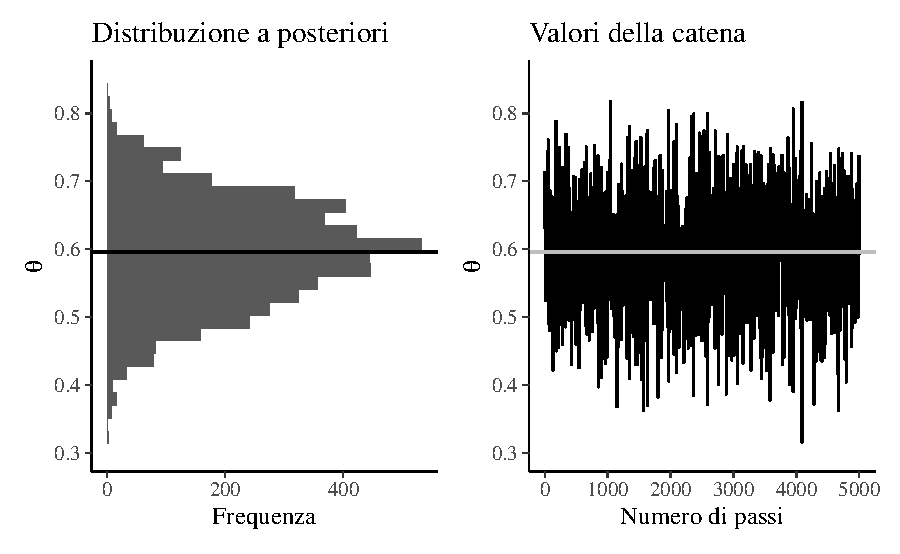
\includegraphics{ds4psy_files/figure-latex/sim-markov-chain-zetsche-1} 

}

\caption{Sinistra. Stima della distribuzione a posteriori della probabilità di una aspettativa futura distorta negativamente per i dati di Zetsche et al. (2019). Destra. Trace plot dei valori della catena di Markov escludendo il periodo di burn-in.}\label{fig:sim-markov-chain-zetsche}
\end{figure}

\hypertarget{input}{%
\subsubsection{Input}\label{input}}

Negli esempi discussi in questo Capitolo abbiamo illustrato l'esecuzione di una singola catena in cui si parte un unico valore iniziale e si raccolgono i valori simulati da molte iterazioni. È possibile che i valori di una catena siano influenzati dalla scelta del valore iniziale. Quindi una raccomandazione generale è di eseguire l'algoritmo di Metropolis più volte utilizzando diversi valori di partenza. In questo caso, si avranno più catene di Markov. Confrontando le proprietà delle diverse catene si esplora la sensibilità dell'inferenza alla scelta del valore di partenza. I software MCMC consentono sempre all'utente di specificare diversi valori di partenza e di generare molteplici catene di Markov.

\hypertarget{stazionarietuxe0}{%
\subsubsection{Stazionarietà}\label{stazionarietuxe0}}

Un punto importante da verificare è se il campionatore ha raggiunto la sua distribuzione stazionaria. La convergenza di una catena di Markov alla distribuzione stazionaria viene detta ``mixing''.

\hypertarget{approx-post-autocor}{%
\subsubsection{Autocorrelazione}\label{approx-post-autocor}}

Informazioni sul ``mixing'' della catena di Markov sono fornite dall'autocorrelazione. L'autocorrelazione misura la correlazione tra i valori successivi di una catena di Markov. Il valore \(m\)-esimo della serie ordinata viene confrontato con un altro valore ritardato di una quantità \(k\) (dove \(k\) è l'entità del ritardo) per verificare quanto si correli al variare di \(k\). L'autocorrelazione di ordine 1 (\emph{lag 1}) misura la correlazione tra valori successivi della catena di Markow (cioè, la correlazione tra \(\theta^{(m)}\) e \(\theta^{(m-1)}\)); l'autocorrelazione di ordine 2 (\emph{lag 2}) misura la correlazione tra valori della catena di Markow separati da due ``passi'' (cioè, la correlazione tra \(\theta^{(m)}\) e \(\theta^{(m-2)}\)); e così via.

L'autocorrelazione di ordine \(k\) è data da \(\rho_k\) e può essere stimata come:

\begin{align}
\rho_k &= \frac{\Cov(\theta_m, \theta_{m+k})}{\Var(\theta_m)}\notag\\
&= \frac{\sum_{m=1}^{n-k}(\theta_m - \bar{\theta})(\theta_{m-k} - \bar{\theta})}{\sum_{m=1}^{n-k}(\theta_m - \bar{\theta})^2} \qquad\text{con }\quad \bar{\theta} = \frac{1}{n}\sum_{m=1}^{n}\theta_m.
\label{eq:autocor}
\end{align}

Per fare un esempio pratico, simuliamo dei dati autocorrelati con la funzione R \texttt{colorednoise::colored\_noise()}:

\begin{Shaded}
\begin{Highlighting}[]
\FunctionTok{suppressPackageStartupMessages}\NormalTok{(}\FunctionTok{library}\NormalTok{(}\StringTok{"colorednoise"}\NormalTok{))}
\FunctionTok{set.seed}\NormalTok{(}\DecValTok{34783859}\NormalTok{)}
\NormalTok{rednoise }\OtherTok{\textless{}{-}} \FunctionTok{colored\_noise}\NormalTok{(}
  \AttributeTok{timesteps =} \DecValTok{30}\NormalTok{, }\AttributeTok{mean =} \FloatTok{0.5}\NormalTok{, }\AttributeTok{sd =} \FloatTok{0.05}\NormalTok{, }\AttributeTok{phi =} \FloatTok{0.3}
\NormalTok{)}
\end{Highlighting}
\end{Shaded}

L'autocorrelazione di ordine 1 è semplicemente la correlazione tra ciascun elemento e quello successivo nella sequenza. Nell'esempio, il vettore \texttt{rednoise} è una sequenza temporale di 30 elementi. Il vettore \texttt{rednoise{[}-length(rednoise){]}} include gli elementi con gli indici da 1 a 29 nella sequenza originaria, mentre il vettore \texttt{rednoise{[}-1{]}} include gli elementi 2:30. Gli elementi delle coppie ordinate dei due vettori avranno dunque gli indici \((1, 2), (2, 3), \dots (29, 30)\) degli elementi della sequenza originaria. La correlazione di Pearson tra i vettori \texttt{rednoise{[}-length(rednoise){]}} e \texttt{rednoise{[}-1{]}} corrisponde dunque all'autocorrelazione di ordine 1 della serie temporale.

\begin{Shaded}
\begin{Highlighting}[]
\FunctionTok{cor}\NormalTok{(rednoise[}\SpecialCharTok{{-}}\FunctionTok{length}\NormalTok{(rednoise)], rednoise[}\SpecialCharTok{{-}}\DecValTok{1}\NormalTok{])}
\CommentTok{\#\textgreater{} [1] 0.3967}
\end{Highlighting}
\end{Shaded}

Il Correlogramma è uno strumento grafico usato per la valutazione della tendenza di una catena di Markov nel tempo. Il correlogramma si costruisce a partire dall'autocorrelazione \(\rho_k\) di una catena di Markov in funzione del ritardo (\emph{lag}) \(k\) con cui l'autocorrelazione è calcolata: nel grafico ogni barretta verticale riporta il valore dell'autocorrelazione (sull'asse delle ordinate) in funzione del ritardo (sull'asse delle ascisse). In \(\R\), il correlogramma può essere prodotto con una chiamata a \texttt{acf()}:

\begin{Shaded}
\begin{Highlighting}[]
\FunctionTok{acf}\NormalTok{(rednoise)}
\end{Highlighting}
\end{Shaded}

\begin{center}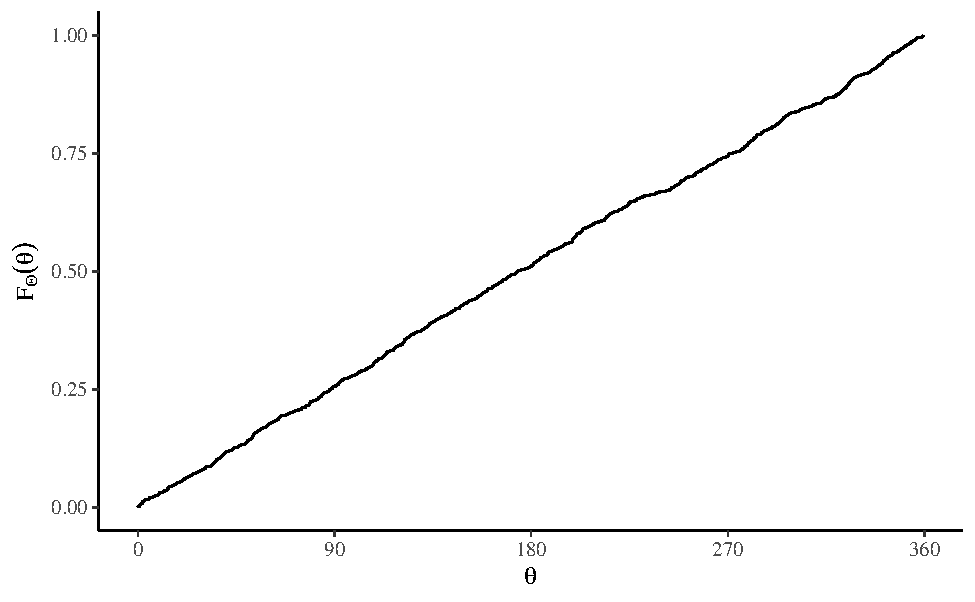
\includegraphics{ds4psy_files/figure-latex/unnamed-chunk-33-1} \end{center}

Il correlogramma precedente mostra come l'autocorrelazione di ordine 1 sia circa pari a 0.4 e diminuisce per lag maggiori; per lag di 4, l'autocorrelazione diventa negativa e aumenta progressivamente fino ad un lag di 8; eccetera.

In situazioni ottimali l'autocorrelazione diminuisce rapidamente ed è effettivamente pari a 0 per piccoli lag. Ciò indica che i valori della catena di Markov che si trovano a più di soli pochi passi di distanza gli uni dagli altri non risultano associati tra loro, il che fornisce conferma del ``mixing'' della catena di Markov, ossia di convergenza alla distribuzione stazionaria. Nelle analisi bayesiane, una delle strategie che consentono di ridurre l'autocorrelazione è quella di assottigliare l'output immagazzinando solo ogni \(m\)-esimo punto dopo il periodo di burn-in. Una tale strategia va sotto il nome di \emph{thinning}.

\hypertarget{test-di-convergenza}{%
\subsubsection{Test di convergenza}\label{test-di-convergenza}}

Un test di convergenza può essere svolto in maniera grafica mediante le tracce delle serie temporali (\emph{trace plot}), cioè il grafico dei valori simulati rispetto al numero di iterazioni. Se la catena è in uno stato stazionario le tracce mostrano assenza di periodicità nel tempo e ampiezza costante, senza tendenze visibili o andamenti degni di nota. Un esempio di \emph{trace plot} è fornito nella figura \ref{fig:sim-markov-chain-zetsche} (destra).

Ci sono inoltre alcuni test che permettono di verificare la stazionarietà del campionatore dopo un dato punto. Uno è il test di Geweke che suddivide il campione, dopo aver rimosso un periodo di burn in, in due parti. Se la catena è in uno stato stazionario, le medie dei due campioni dovrebbero essere uguali. Un test modificato, chiamato Geweke z-score, utilizza un test \(z\) per confrontare i due subcampioni ed il risultante test statistico, se ad esempio è più alto di 2, indica che la media della serie sta ancora muovendosi da un punto ad un altro e quindi è necessario un periodo di burn-in più lungo.

\hypertarget{commenti-e-considerazioni-finali-1}{%
\section*{Commenti e considerazioni finali}\label{commenti-e-considerazioni-finali-1}}


In generale, la distribuzione a posteriori dei parametri di un modello statistico non può essere determinata per via analitica. Tale problema, invece, viene affrontato facendo ricorso ad una classe di algoritmi per il campionamento da distribuzioni di probabilità che sono estremamente onerosi dal punto di vista computazionale e che possono essere utilizzati nelle applicazioni pratiche solo grazie alla potenza di calcolo dei moderni computer. Lo sviluppo di software che rendono sempre più semplice l'uso dei metodi MCMC, insieme all'incremento della potenza di calcolo dei computer, ha contribuito a rendere sempre più popolare il metodo dell'inferenza bayesiana che, in questo modo, può essere estesa a problemi di qualunque grado di complessità.

Nel 1989 un gruppo di statistici nel Regno Unito si pose il problema di simulare le catene di Markov su un personal computer. Nel 1997 ci riuscirono con il primo rilascio pubblico di un'implementazione Windows dell'inferenza bayesiana basata su Gibbs sampling, detta BUGS. Il materiale presentato in questo capitolo descrive gli sviluppi contemporanei del percorso che è iniziato in quel periodo.

  \bibliography{refs.bib,book.bib,packages.bib}

\printindex

\end{document}
